%% Based on a TeXnicCenter-Template by Gyorgy SZEIDL.
%%%%%%%%%%%%%%%%%%%%%%%%%%%%%%%%%%%%%%%%%%%%%%%%%%%%%%%%%%%%%

%------------------------------------------------------------
%
%\documentclass{amsart}
\documentclass[a4paper,oneside,12pt,english]{report}
\usepackage{url}
\usepackage[pdftex]{color,graphicx}


\usepackage{amsmath}%
\usepackage{amsfonts}%
\usepackage{amssymb}%
\usepackage{graphicx}


\usepackage{tikz}



\usepackage[backref=false]{hyperref}
\hypersetup{plainpages = false,
              breaklinks=true,
              %a4paper=true,
              linktocpage,
              colorlinks   = true, %Colours links instead of ugly boxes
              urlcolor     = blue, %Colour for external hyperlinks
              linkcolor    = blue, %Colour of internal links
              citecolor   = red, %Colour of citations              pdfauthor={Niko Brummer},
              pdfauthor={Niko Brummer},
              %pdfpagemode=None,
              pdfstartpage=1, 
              pdfstartview=FitH,  
              pdfkeywords={}}

%
%----------------------------------------------------------
% This is a sample document for the AMS LaTeX Article Class
% Class options
%        -- Point size:  8pt, 9pt, 10pt (default), 11pt, 12pt
%        -- Paper size:  letterpaper(default), a4paper
%        -- Orientation: portrait(default), landscape
%        -- Print size:  oneside, twoside(default)
%        -- Quality:     final(default), draft
%        -- Title page:  notitlepage, titlepage(default)
%        -- Start chapter on left:
%                        openright(default), openany
%        -- Columns:     onecolumn(default), twocolumn
%        -- Omit extra math features:
%                        nomath
%        -- AMSfonts:    noamsfonts
%        -- PSAMSFonts  (fewer AMSfonts sizes):
%                        psamsfonts
%        -- Equation numbering:
%                        leqno(default), reqno (equation numbers are on the right side)
%        -- Equation centering:
%                        centertags(default), tbtags
%        -- Displayed equations (centered is the default):
%                        fleqn (equations start at the same distance from the right side)
%        -- Electronic journal:
%                        e-only
%------------------------------------------------------------
% For instance the command
%  \documentclass[a4paper,12pt,reqno]{amsart}
% ensures that the paper size is a4, fonts are typeset at the size 12p
% and the equation numbers are on the right side
%


%\usetikzlibrary{external}
%\tikzexternalize
%\tikzset{external/force remake=true}  
%Die werk nie, maar Albert s^e: ek moes ook pdflatex met die hand loop om die figure te genereer.  Die --shell-escape flaggie is nodig om daardie external command uit te voer.  
% Jy kan "pdflatex --shell-escape paper.tex" in die konsole uitvoer, of probeer om "--shell-escape" in jou LaTeX editor se pdflatex configurasie as argument te spesifiseer.

\usetikzlibrary{bayesnet}
\renewcommand{\edge}[3][]{ %
  % Connect all nodes #2 to all nodes #3.
  \foreach \x in {#2} { %
    \foreach \y in {#3} { %
      \path (\x) edge [->,#1] (\y) ;%
      %\draw[->,#1] (\x) -- (\y) ;%
    } ;
  } ;
}
\newcommand{\uedge}[3][]{ %
  % Connect all nodes #2 to all nodes #3.
  \foreach \x in {#2} { %
    \foreach \y in {#3} { %
      \path (\x) edge [-,#1] (\y) ;%
      %\draw[->,#1] (\x) -- (\y) ;%
    } ;
  } ;
}



\usetikzlibrary{arrows,shapes,backgrounds,positioning,fit}

% Caches tikz figures as PDF on disk. 
% Needs --shell-escape on pdflatex commandline, or for TexicCenter, see here: https://tex.stackexchange.com/questions/222632/how-to-do-shell-escape-in-texniccenter
\usetikzlibrary{external}
\tikzexternalize

\usepackage{upgreek}

\usepackage{enumerate}
\usepackage{titlepic}

%------------------------------------------------------------
%\numberwithin{equation}{section}

\def\alphavec{\boldsymbol{\alpha}}
\def\betavec{\boldsymbol{\beta}}
\def\lambdavec{\boldsymbol{\lambda}}
\def\gammavec{\boldsymbol{\gamma}}
\def\Lambdamat{\boldsymbol{\Lambda}}
\def\pivec{\boldsymbol{\Pi}}
\def\Vmat{\mathbf{V}}

\def\zvec{\mathbf{z}}
\def\hvec{\mathbf{h}}
\def\vvec{\mathbf{v}}
\def\wvec{\mathbf{w}}

\def\ND{\mathcal{N}}

\DeclareMathOperator{\detnt}{det}
\DeclareMathOperator{\chol}{chol}
\DeclareMathOperator{\diag}{diag}
\DeclareMathOperator{\trace}{tr}
\DeclareMathOperator{\abs}{abs}
\DeclareMathOperator*{\argmax}{argmax}
\DeclareMathOperator*{\argmin}{argmin}

\DeclareMathOperator{\logit}{logit}

\def\expvb#1#2{\left\langle#1\right\rangle_{#2}}
\def\expv#1#2{\bigl\langle#1\bigr\rangle_{#2}}
\def\expp#1{\bigl\langle#1\bigr\rangle}



\def\KL#1#2{D_{KL}\bigl[#1\|#2\bigr]}

\def\LRT#1#2{\text{LR}(\text{#1},\text{#2})}
\def\R{\mathbb{R}}
\def\detm#1{\lvert#1\rvert}

\def\Xset{\mathcal{X}}
\def\Lset{\mathcal{L}}
\def\Zset{\mathcal{Z}}
\def\Yset{\mathcal{Y}}
\def\model{\mathcal{M}}


\def\Lmat{\mathbf{L}}
\def\Bmat{\mathbf{B}}
\def\Wmat{\mathbf{W}}
\def\Cmat{\mathbf{C}}
\def\Dmat{\mathbf{D}}
\def\Fmat{\mathbf{F}}
\def\Gmat{\mathbf{G}}
\def\Hmat{\mathbf{H}}
\def\Smat{\mathbf{S}}
\def\Emat{\mathbf{E}}
\def\Imat{\mathbf{I}}
\def\Ymat{\mathbf{Y}}
\def\Xmat{\mathbf{X}}
\def\Rmat{\mathbf{R}}
\def\Tmat{\mathbf{T}}
\def\Mmat{\mathbf{M}}
\def\Nmat{\mathbf{N}}
\def\Kmat{\mathbf{K}}
\def\Gmat{\mathbf{G}}

\def\yvec{\mathbf{y}}
\def\svec{\mathbf{s}}
\def\nvec{\mathbf{n}}
\def\xvec{\mathbf{x}}
\def\mvec{\mathbf{m}}
\def\fvec{\mathbf{f}}
\def\gvec{\mathbf{g}}
\def\rvec{\mathbf{r}}
\def\muvec{\boldsymbol{\mu}}
\def\phivec{\boldsymbol{\phi}}


\def\avec{\mathbf{a}}
\def\bvec{\mathbf{b}}



\def\Rset{\mathcal{R}}
\def\Sset{\mathcal{S}}
\def\Tset{\mathcal{T}}
\def\Eset{\mathcal{E}}
\def\Zset{\mathcal{Z}}






\def\yhat{\hat{\mathbf{y}}}
\def\nulvec{\boldsymbol{0}}
\def\logdet#1{\log\detm{#1}}
\def\const{\text{const}}


%symmetric matrix inversion lemma
\newcommand{\inv}[1]{%  
\ifx{#1}{\Imat}           %this test fails
  #1
\else
  {#1}^{-1}
\fi
}
%\newcommand{\SMILP}[3][\Imat]{{#1}^{-1}+{#3}'{#2}^{-1}{#3}}
\newcommand{\SMILP}[3][\Imat]{\inv{#1}+{#3}'{#2}^{-1}{#3}}
\newcommand{\SMIL}[3]{{#2}^{-1}-{#2}^{-1}{#3}{#1}^{-1}{#3}'{#2}^{-1}}


\def\Isetg#1#2#3{\{#1\}_{#2}^{#3}}
\def\Iset#1#2#3{\{#1_{#2}\}_{#2=1}^{#3}}

\def\funcdef#1#2#3{#1:#2\to#3}
\def\Fset{\mathcal{F}}
\def\C{\mathbb{C}}
\def\Cset{\mathcal{C}}

%\def\FT#1{\Fset\{#1\}}
%\def\IFT#1{\Fset^{-1}\{#1\}}
\newcommand\FT[2][]{\Fset_{#1}\{#2\}}
\newcommand\CT[2][]{\Cset_{#1}\{#2\}}
\def\IFT#1{\Fset^{-1}\{#1\}}

\def\conj#1{\overline{#1}}


\begin{document}

\tikzstyle{every picture}+=[remember picture]


\tikzstyle{cbox} = [rectangle,draw=blue!100,thick,align=center,rounded corners = 3pt]
\tikzstyle{lbox} = [rectangle,draw=blue!100,thick,align=left,rounded corners = 3pt]
\tikzstyle{ccircle} = [circle,draw=blue!100,thick,align=center,inner sep = 0]
\tikzstyle{ctext} = [rectangle,align=center,inner sep = 4pt]
\tikzstyle{ltext} = [rectangle,align=left,inner sep = 4pt]
\tikzstyle{solder} = [circle,draw,fill,inner sep = 0, minimum size = 6pt]


\hypersetup{pageanchor=false}


\title{Meta-embeddings: a probabilistic generalization of embeddings in machine learning}
\author{Niko Br\"ummer\footnote{Corresponding author: \url{niko.brummer@gmail.com}. The other authors are in alphabetical order.}~, Luk\'{a}\v{s} Burget, Paola Garcia, \\ Old\v{r}ich Plchot, Johan Rohdin, Daniel Romero,\\ David Snyder, Themos Stafylakis, Jes\'us Villalba}
\date{JHU HLTCOE 2017 SCALE Workshop}

\titlepic{
\begin{tikzpicture}[xscale=1.5,yscale=1.5,thick]
\node[solder,green] at(0,0) (bottom) {};
%
\node[solder,red] at(-2.5,1) (n1_23_4) {};
\node[solder] at(-1.5,1) (n14_2_3) {};
\node[solder,blue] at(-0.5,1) (n1_24_3) {};
\node[solder,blue] at(0.5,1) (n13_2_4) {};
\node[solder,green] at(1.5,1) (n12_3_4) {};
\node[solder] at(2.5,1) (n1_2_34) {};
\draw[green] (bottom) to (n1_23_4);
\draw (bottom) to (n14_2_3);
\draw (bottom) to (n13_2_4);
\draw[green] (bottom) to (n12_3_4);
\draw (bottom) to (n1_2_34);
\draw (bottom) to (n1_24_3);
%
\node[solder,red] at(-3,3) (n14_23) {};
\node[solder] at(-2,3) (n1_234) {};
\node[solder,red] at(-1,3) (n124_3) {};
\node[solder,blue] at(0,3) (n13_24) {};
\node[solder] at(1,3) (n123_4) {};
\node[solder] at(2,3) (n134_2) {};
\node[solder] at(3,3) (n12_34) {};
\draw[red] (n14_23) to (n1_23_4);
\draw (n14_23) to (n14_2_3);
\draw (n1_234) to (n1_2_34);
\draw (n1_234) to (n1_23_4);
\draw (n1_234) to (n1_24_3);
\draw (n124_3) to (n14_2_3);
\draw (n124_3) to (n1_24_3);
\draw[green] (n124_3) to (n12_3_4);
\draw[blue] (n13_24) to (n1_24_3);
\draw[blue] (n13_24) to (n13_2_4);
\draw (n123_4) to (n12_3_4);
\draw (n123_4) to (n13_2_4);
\draw (n123_4) to (n1_23_4);
\draw (n134_2) to (n14_2_3);
\draw (n134_2) to (n1_2_34);
\draw (n134_2) to (n13_2_4);
\draw (n134_2) to (n14_2_3);
\draw (n134_2) to (n1_2_34);
\draw (n134_2) to (n13_2_4);
\draw (n12_34) to (n1_2_34);
\draw (n12_34) to (n12_3_4);
%
\node[solder,red] at(0,4) (top) {};
\draw[red] (top) to (n14_23);
\draw (top) to (n1_234);
\draw[red] (top) to (n124_3);
\draw (top) to (n13_24);
\draw (top) to (n123_4);
\draw (top) to (n134_2);
\draw (top) to (n12_34);
\end{tikzpicture}
}


\maketitle



\hypersetup{pageanchor=true}


\tableofcontents
\listoffigures

\chapter{Introduction}

\emph{Embeddings} are familiar in modern machine learning. Neural nets to extract word embeddings\footnote{\url{en.wikipedia.org/wiki/Word_embedding}} were already proposed in 2000 by Bengio~\cite{Bengio_word_embedding}. Now embeddings are used more generally, for example in state-of-the-art face recognition, e.g.\ Facenet~\cite{Facenet}.

Embeddings are becoming popular also in speech and speaker recognition. In Interspeech 2017, eighteen papers had the word `embedding' in the title.\footnote{\url{www.interspeech2017.org/program/technical-program/}.} In speaker recognition and spoken language recognition, we have been using i-vectors, a precursor to embeddings, for almost a decade~\cite{ivector-Brighton,ivec,BUT_ivector_language}. More general embeddings are now appearing in speaker recognition, see for example the Voxceleb paper~\cite{Voxceleb} and David Snyder's work~\cite{end2end,DSIS17}. A new embedding method for language recognition is proposed in~\cite{LIMSI_Language_embedding}. 
 
Input patterns (sequences of acoustic feature vectors, images, text, \ldots) live in large, complex spaces, where probability distributions and geometrical concepts such as distance are difficult to formulate. Embeddings extracted from the input patterns live in simpler spaces, e.g.\ $\R^d$ (multidimensional Euclidean space), where distance is naturally defined and can be put to work to compare patterns. 

At the Johns Hopkins HLTCOE SCALE 2017 Workshop\footnote{\url{http://hltcoe.jhu.edu/research/scale/scale-2017}} one of the topics of interest was embeddings for speaker recognition. During the workshop, the idea to generalize to \emph{meta-embeddings} was conceived. At the time of the writing of this document, we are still developing the theory and no code has been written, nor have any experiments been performed. This document describes the theory.    

We envisage that meta-embeddings could be widely applicable to a variety of machine learning or pattern recognition problems, but we shall make our discussion concrete by using the language of automatic speaker verification/recognition. To interpret everything (say) as face recognition, just do \emph{recording}$\,\mapsto\,$\emph{image} and \emph{speaker}$\,\mapsto\,$\emph{face}, and so on \ldots.

\section{Meta-embeddings}
An important concept used throughout this document is that of the \emph{hidden identity variable}---a hypothetical, multidimensional variable that ideally contains all of the information that distinguishes one speaker/face/individual from others. In speaker recognition, the hidden \emph{speaker identity variable} is well known from the work of Patrick Kenny in JFA~\cite{JFA} and PLDA~\cite{HTPLDA}. Similar identity variables appeared in earlier face recognition applications of PLDA~\cite{PLDA-IOFFE, PLDA-Prince, PLDA-Li}.

We argue that the way embeddings are currently treated, essentially makes them \emph{point estimates of hidden variables}. We propose instead to let the identity variables---and therefore the embeddings---remain hidden and to instead extract \emph{meta-embeddings}, which are probabilistic representations of what the values of the hidden variables might be. For example, if the embedding lives in $\R^d$, then the meta-embedding could be in the form of a multivariate normal distribution, where the mean could act as point estimate, but where there is also a covariance matrix that quantifies the uncertainty around the mean. 

Quantifying the uncertainty is very important if the recognizer is to be applicable to variable and sometimes challenging conditions. In speaker recognition, a short, noisy, narrow-band recording should leave much more uncertainty about the speaker than a long, clean, wideband recording. In face recognition, compare a well-lit, high resolution, full-frontal face image to a grainy, low resolution, partly occluded face. In fingerprint recognition, compare a clean, high-resolution ten-print, to a single, distorted, smudged fingermark retrieved from a crime scene.    

The idea to represent the uncertainty is not novel. Indeed, it is \emph{obvious} that to do things properly, we must take the uncertainty into account. The problem is that it turns out to be difficult to do in practice. 
\begin{itemize}
	\item Part of the problem is computational. For example, a point estimate for an identity variable in $\R^d$ can be represented as a $d$-dimensional vector. But for a multivariate normal meta-embedding, the covariance is a $d$-by-$d$ matrix, which is more expensive to store and manipulate. 
	\item Then there is the added complication that covariance matrices have to be positive definite. If we use a neural net to compute our uncertainty for us, we have to specially structure the neural net to respect this requirement. 
	\item But the problem has another facet---if a neural net manufactures meta-embeddings for us, how do we know that the uncertainty thus represented is reasonable? Given meta-embeddings extracted from some supervised database, what criterion can we apply to measure the goodness of the information and the uncertainty they contain? Such criteria are important, because we need them for discriminative training of our neural nets.
\end{itemize}
This document will provide some suggestions for tackling the above problems.\\ 

\noindent The main purpose of the document is however to show that the meta-embeddings are themselves embeddings in the sense that they live in a vector space, equipped with geometric and algebraic structure that can be employed to compute probabilistic recognition scores (likelihood ratios). The hope is that the theoretical part of this document will help to provide the structure to guide further research into finding better solutions for the practical problems of working with this kind of uncertainty.    



\section{Prior work}
In~\cite{Vilnis}, Gaussian embeddings are proposed to represent uncertainty. To be expanded, \ldots\\

\noindent Mention uncertainty propagation in i-vectors\cite{Uncertainty-Sandro, Uncertainty-Patrick, Uncertainty-Themos, Uncertainty-Bilbao}, \ldots 

\chapter{Distillation of meta-embeddings from independence assumptions}
\label{chap:fp}
In this chapter we use probability theory and some basic independence assumptions to motivate and derive the concept of meta-embeddings.  

We use speaker recognition terminology, but everything is applicable more widely (images, etc. \ldots). Our inputs are \emph{voice recordings}, each assumed to contain a single speaker. Recordings can have various representations, i-vectors, sequences of feature vectors, the raw speech samples, etc. \ldots. At the writing of this document, recordings represented as feature vector sequences are of primary interest.  

In general, we will be interested in \emph{sets} of recordings, ranging from the set of all the recordings in a training database, down to just a pair of recordings in a verification trial. We represent a set of $n$ recordings as:
\begin{align*}
\Rset &=\{r_1,r_2,\ldots,r_n\}
\end{align*}
We shall work with hypotheses about how such sets of recordings are partitioned w.r.t.\ speaker and we shall make use of independence assumptions conditioned on these hypotheses. 

\section{Independence assumptions}
\label{sec:IS}
We base everything that follows on a pair of simple independence assumptions: 
\begin{itemize}
	\item Multiple recordings of the same speaker are \emph{exchangeable}.
	\item Recordings of different speakers are \emph{independent}. 
\end{itemize}
Almost all current probabilistic solutions in speaker recognition---also PLDA---make use of these assumptions. While these assumptions are mathematically convenient, in the real world they are not exactly true: 
\begin{itemize}
	\item The speech of any speaker will change over a time span of years and recordings made over such a period will not be exchangeable. 
	\item The independence assumption between different speakers can only apply if our recognizer is sufficiently well trained: The recognizer has to have been exposed to so much speech, that only the speech of a new speaker itself can provide information about that speaker.
\end{itemize}
As long as we understand the limitations imposed by our assumptions, we can proceed.  \\

\noindent In what follows, we use the notation $H_1$ for the hypothesis that the set of recordings of interest, $\Rset=\{r_1,\ldots,r_n\}$, were all spoken by the same (one) speaker. For the hypothesis that they were spoken by $m$ different speakers, we use $H_m$. Exchangeability means:
\begin{align*}
P(\Rset\mid H_1) &= P(r_1,r_2\ldots,r_n\mid H_1) = P(r_2,r_1,\ldots,r_n\mid H_1) = \cdots
\end{align*}
where the joint probability does not depend on the order of the recordings. According to De Finetti's exchangeability theorem,\footnote{\url{en.wikipedia.org/wiki/Exchangeable_random_variables}} the only way to obtain exchangeability is to introduce some hidden variable, say $\zvec\in\Zset$, such that the recordings are \emph{conditionally independent} given $\zvec$. Marginalizing over $\zvec$ w.r.t.\ some prior distribution $\pi(\zvec)$, gives the exchangeable joint distribution~\cite{Chow}:  
\begin{align}
\label{eq:exch}
P(\Rset\mid H_1) &= \expv{\prod_{i=1}^n P(r_i\mid \zvec)}{\zvec\sim\pi}
\end{align}
where the angle brackets denote expectation---for continuous $\zvec$, this could be written as an integral and for discrete $\zvec$ as a summation. By this marginalization, we are inducing dependence between recordings of the same speaker, while retaining exchangeability. \emph{We do need this dependence, otherwise speaker recognition would be impossible!}\\

\noindent Let $\Rset_1,\Rset_2,\ldots,\Rset_m$ be a number of non-overlapping sets of recordings, spoken respectively by $m$ different speakers. The between-speaker independence assumption gives:
\begin{align}
\label{eq:iid}
P(\Rset_1,\ldots,\Rset_m\mid\text{$m$ speakers}) &= \prod_{i=1}^m P(\Rset_i\mid H_1) = \prod_{i=1}^m \expv{\prod_{r\in\Rset_i} P(r\mid\zvec)}{\zvec\sim\pi}   
\end{align}
where we have expanded $P(\Rset_i\mid H_1)$ using~\eqref{eq:exch}.

According to this model, the hidden variable, $\zvec\in\Zset$, contains everything that is to be known about recordings of a speaker. Patrick Kenny calls $\zvec$ the \emph{speaker identity variable}. At this stage, we are not committing ourselves to the nature of the hidden variables and therefore we leave $\Zset$ undefined---after all, $\zvec$ is hidden so there is much freedom in choosing its nature. (If you need something concrete to shape your thoughts, $\Zset=\R^d$ is a good choice.) 

Think of the identity variable, $\zvec$, as the ideal embedding that an oracle could extract. If we were given $\zvec$, the problem would be instantly solved. Unfortunately, there is noise, distortion, occlusion and all kinds of other mechanisms that induce uncertainty, so we can never exactly extract $\zvec$. Let's not pretend that we can do this. Let us not extract some point-estimate for $\zvec$ and call that our embedding. Let's instead extract a \emph{meta-embedding}, which is \emph{information about} the ideal embedding, $\zvec$, where the information has a probabilistic form. We derive this form below.


\section{Speaker identity likelihood functions}
\label{sec:silf}
Given a pair of recordings, $\Rset=\{r,r'\}$, we can answer the question of whether they belong to the same speaker or not in terms of the \emph{likelihood-ratio (LR)}~\cite{NikoCSL}:
%\begin{align}
%\begin{split}
%\frac{P(r,r'\mid H_1)}{P(r,r'\mid H_2)} &= \frac{\expv{P(r\mid\zvec)\;P(r'\mid\zvec)}{\zvec\sim\pi}}{P(r)\;P(r')} \\
%&= \expv{\frac{P(r\mid\zvec)}{P(r)}\;\frac{P(r'\mid\zvec)}{P(r')}}{\zvec\sim\pi}  \\
%&= \expv{\frac{P(\zvec\mid r)}{\pi(\zvec)}\;\frac{P(\zvec\mid r')}{\pi(\zvec)}}{\zvec\sim\pi}  \\
%\end{split}
%\end{align}
\begin{align}
\label{eq:SLR}
\begin{split}
\frac{P(r,r'\mid H_1)}{P(r,r'\mid H_2)} &= \frac{\expv{P(r\mid\zvec)\;P(r'\mid\zvec)}{\zvec\sim\pi}}
{\expv{P(r\mid\zvec)}{\zvec\sim\pi}\;\expv{P(r'\mid\zvec)}{\zvec\sim\pi}} \\
&= \frac{\expv{kP(r\mid\zvec)\;k'P(r'\mid\zvec)}{\zvec\sim\pi}}
{\expv{kP(r\mid\zvec)}{\zvec\sim\pi}\;\expv{k'P(r'\mid\zvec)}{\zvec\sim\pi}} \\
&= \frac{\expv{f_r(\zvec)\;f_{r'}(\zvec)}{\zvec\sim\pi}}
{\expv{f_r(\zvec)}{\zvec\sim\pi}\;\expv{f_{r'}(\zvec)}{\zvec\sim\pi}}
\end{split}
\end{align}
where we have defined the \emph{speaker identity likelihood functions}: 
\begin{align}
f_r(\zvec)&=kP(r\mid\zvec)& \text{and} && f_{r'}(\zvec)&=k'P(r'\mid\zvec),
\end{align}
where $k,k'>0$ are arbitrary constants that may depend on $r,r'$, but not on $\zvec$. Notice that the LR depends on the data ($r,r'$) only via $f_r$ and $f_{r'}$. The speaker information in $r$ is represented by the \emph{whole function} 
$$f_r:\Zset\to\R$$ 
rather than by the function value $f_r(\zvec)$ at some particular value of $\zvec$ (remember $\zvec$ is hidden and we are never given a fixed value for it).

The full speaker information cannot be represented by some estimate of $\zvec$.  We could for example use $\hat\zvec = \argmax f_r(\zvec)$ as a maximum-likelihood point-estimate for $\zvec$, but that would be throwing information away. The full information about the speaker is contained in the whole function, $f_r$.

The representation of the speaker information can be further understood by noticing that $f_r$ and $f_{r'}$ represent $r,r'$ in any posteriors for the speaker identity variable, for example:
\begin{align}
P(\zvec\mid r, \pi) &= \frac{\pi(\zvec)f_r(\zvec)}{\expv{f_r(\zvec')}{\zvec'\sim\pi}}
\end{align}
and if $r$ and $r'$ are known to be of the same speaker, then:
\begin{align}
P(\zvec\mid r,r',H_1,\pi) &= \frac{\pi(\zvec)f_r(\zvec)f_{r'}(\zvec)}{\expv{f_r(\zvec')f_{r'}(\zvec')}{\zvec'\sim\pi}}
\end{align}


\section{The general case}
\label{sec:general}
Our speaker identity likelihood functions are applicable more generally than just to pairs of recordings. Under the independence assumptions of section~\ref{sec:IS}, speaker identity likelihood functions can be used to answer \emph{any} question that can be formulated in terms of partitioning a set of recordings according to speaker~\cite{SPP}. Let $\Rset=\{r_1,\ldots,r_n\}$ be a set of recordings and let $A: \Sset_1,\Sset_2,\ldots,\Sset_m\subseteq\{1,2,\ldots,n\}$ be a hypothesized partition of $\Rset$ into subsets belonging to $m\ge1$ different hypothesized speakers.\footnote{The subsets are non-empty, non-overlapping and their union equals $\{1,2,\ldots,n\}$. We allow $m=1$, in which case $\Sset_1=\Rset$.} Similarly, let $B: \Sset'_1,\ldots,\Sset'_{m'}$ be a different hypothesized partition, having $m'$ hypothesized speakers. $A$ and $B$ are labels that refer to the two alternate partitioning hypotheses. Using within-speaker exchangeability and between-speaker independence, the LR comparing $A$ to $B$ is:
\begin{align}
\label{eq:generalLR}
\begin{split}
\frac{P(\Rset\mid A)}{P(\Rset\mid B)} &=
\frac{\prod_{i=1}^m \expvb{\prod_{j\in\Sset_i} P(r_j\mid\zvec)}{\zvec\sim\pi}}
{\prod_{i=1}^{m'} \expvb{\prod_{j\in\Sset'_i} P(r_j\mid\zvec)}{\zvec\sim\pi}} \\
&= \frac{\prod_{i=1}^m \expvb{\prod_{j\in\Sset_i} f_j(\zvec)}{\zvec\sim\pi}}
{\prod_{i=1}^{m'} \expvb{\prod_{j\in\Sset'_i} f_j(\zvec)}{\zvec\sim\pi}} 
\end{split}
\end{align}
where, as above, the \emph{speaker identity likelihood function} extracted from $r_j$ is:
\begin{align}
f_j(\zvec)=k_jP(r_j\mid\zvec)
\end{align}
The last equality in~\eqref{eq:generalLR} follows because the arbitrary scaling constants, $\{k_j\}_{j=1}^n$, are the same in the numerator and denominator and cancel. This LR form is convenient because of this cancellation.

Any kind of speaker recognition problem that can be expressed in terms of partitioning recordings according to speaker, can be scored at runtime via likelihood-ratios of the form~\eqref{eq:generalLR}. We shall show some examples below.  Moreover, any discriminative training criteria that are expressed as functions of the LR scores can then also be expressed in terms of~\eqref{eq:generalLR}. In summary: 
\begin{quote}
\emph{For discriminative speaker recognition, all scoring and training calculations can be expressed in terms of the speaker identity likelihood functions.} 
\end{quote}
To better appreciate this generality, we shall present some examples in the next section.

Again, for readers that are comfortable with the idea that probability distributions convey information~\cite{PTLOS}, the speaker identity likelihood functions are closely associated with posteriors for $\zvec$. Any such posterior, conditioned on a number of recordings of a speaker indexed by $\Sset$, can be computed as:
\begin{align}
P(\zvec\mid \Rset,\Sset,H_1,\pi) &=\frac{\pi(\zvec)\prod_{j\in\Sset}f_j(\zvec)}{\expvb{\prod_{j\in\Sset}f_j(\zvec')}{\zvec'\sim\pi}}
\end{align}
The likelihood function, $f_j$, or indeed a product of any number of them, can be regarded as a \emph{raw} form of posterior distribution for $\zvec$. We use the term raw, because the likelihood function is independent of the choice of prior, $\pi$, and is also un-normalized. Nevertheless, $f_j$ contains all the speaker information that a given probabilistic model could extract from $r_j$.




\section{Examples}
\label{sec:examples}
The examples below should aid understanding of the meaning and applications of~\eqref{eq:generalLR}. We will frequently refer back to these examples in the rest of this document.\\

\noindent\textbf{Simple verification.} Let $\Rset=\{r_1,r_2\}$, $A:\Sset_1=\{1,2\}$ and $B:\Sset'_1=\{1\},\Sset'_2=\{2\}$. Then $\frac{P(\Rset\mid A)}{P(\Rset\mid B)}$ is the canonical (single-enroll) speaker verification LR.\\

\noindent\textbf{Multi-enroll verification.} Let $\Rset=\{r_1,r_2,r_3\}$, $A:\Sset_1=\{1,2,3\}$ and $B:\Sset'_1=\{1,2\},\Sset'_2=\{3\}$. Then $\frac{P(\Rset\mid A)}{P(\Rset\mid B)}$ is the speaker verification LR, with enrollment recordings $r_1,r_2$ and test recording $r_3$.\\

\noindent\textbf{Open set classification.} Let $\Rset=\{r_1,\ldots,r_n\}$ be partitioned into $m$ speakers, indexed by $\Sset_1,\ldots,\Sset_m\subseteq\{1,\ldots,n\}$. Let $r'\ne\Rset$ be an additional (test) recording. For $1\le i\le m$, let $A_i$ be the hypothesis that $r'$ is spoken by speaker $i$, as indexed by $\Sset_i$. Let $A_{m+1}$ be the hypothesis that there are $m+1$ speakers: $m$ of them indexed by $\Sset_1,\ldots,\Sset_m$ and $r'$ spoken by a new speaker.  Then we can score the open-set speaker classification problem as follows: For $1\le i\le m+1$, the likelihood\footnote{The numerator of $L_i$ by itself, $P(\Rset,r'\mid A_i)$, could also serve as likelihood for $A_i$. Since the denominator is independent of $i$, the normalized ratio, $L_i$, is still a valid likelihood for $A_i$, with the advantage that the troublesome data-dependent constants cancel.} for $A_i$ is 
\begin{align}
L_i=\frac{P(\Rset,r'\mid A_i)}{P(\Rset,r'\mid A_{m+1})}
\end{align}
Notice that likelihood that $r'$ was spoken by a new speaker is just $L_{m+1}=1$. Assuming some hypothesis prior, $P(A_i)$, the hypothesis posterior is:
\begin{align}
P(A_i\mid\Rset,r') &= \frac{P(A_i)L_i}{\sum_{j=1}^{m+1} P(A_j)L_j}
\end{align}\\
	
\noindent\textbf{Agglomerative hierarchical clustering.} Let $\Rset=\{r_1,\ldots,r_n\}$ be partitioned into $m$ hypothesized speakers, indexed by $A:\Sset_1,\ldots,\Sset_m\subseteq\{1,\ldots,n\}$. For $1\le i,j\le m$ and $i\ne j$, let $B_{ij}$ be the hypothesis that the speakers are correctly indexed as given by $A$, except that the recordings indexed by $\Sset_i$ and $\Sset_j$ are from the same speaker. That is, if we accept hypothesis $B_{ij}$, then we should reduce the number of speakers to $m-1$ and merge $\Sset_i$ and $\Sset_j$. We let 
\begin{align}
\label{eq:LR_AHC}
L_{ij}=\frac{P(\Rset\mid B_{ij})}{P(\Rset\mid A)}
\end{align}
be the (conveniently normalized) likelihood for hypothesis $B_{ij}$,  while the likelihood for hypothesis $A$ is just 1. These likelihood scores can be used as part of an iterative, greedy optimization\footnote{Finding the global optimum is apparently hopelessly intractable. For a set of $n=75$ recordings, we already have that the number of possible ways to partition this set exceeds the number of atoms (about $10^{80}$) in the observable universe.} procedure (agglomerative hierarchical clustering) to find a partition of $\Rset$ according to speaker, with high posterior probability. \\


\noindent
\textbf{Summary.} All of these examples are scored using likelihood ratios of the form~\eqref{eq:generalLR} and are therefore dependent on the data only via the speaker identity likelihood functions. 

We have so far demonstrated that $f_j$ qualifies as an embedding in the sense that it contains all of the relevant information in $r_j$. In what follows we shall refer to $\zvec$ as the (hidden, ideal) \emph{embedding}, while the $f_j$ are our \emph{meta-embeddings}. 

It remains to be shown in the next chapter that these meta-embeddings live in a space with useful algebraic and geometric structure.
	
	
\chapter{The structure of meta-embedding space}
Classical embeddings in machine learning live in finite-dimensional, Euclidean space, $\R^d$. When equipped with the standard scalar product, vector addition, dot-product and Euclidean distance, $\R^d$ is a vector space, inner-product space, metric space, Hilbert space, etc.\ Our meta-embeddings, the functions $f_j$, live in a slightly generalized space, which is still a vector space, inner product space, metric space and (subject to regularity conditions) a Hilbert space. 

Depending on the nature of the hidden variable, $\zvec\in\Zset$, our meta-embeddings might live in a space with very high, or even infinite dimensionality. In the theory that follows, everything can be more elegantly described in this high/infinite-dimensional space, but in practice---to be discussed in the next chapter---we will consider various finite, tractable representations of our meta-embeddings.

In this chapter we explore first the geometric (vector space) properties of meta embeddings that establish concepts such as length, distance and angle. The vector space operations include addition, scalar multiplication and inner product. Next we enrich the vector space by introducing another (elementwise) multiplicative operator, which then forms an algebra. We explain some of the properties of this algebra and finally show how these algebraic manipulations can be used to compute likelihood-ratios of the form~\eqref{eq:generalLR}.

The chapter concludes with a simple graphical example to aid understanding.

\section{Geometric properties}


Let $\R^\Zset$ denote the space of all possible functions from $\Zset$ to $\R$ and let our meta-embeddings live in $\Fset$, where $\Fset\subset\R^{\Zset}$. We need to confine meta-embeddings to some subset of $\R^\Zset$ in order to exclude all kinds of pathological functions and to ensure that the operations defined on meta-embeddings are well behaved. Since our meta-embeddings are likelihoods, the function values are always non-negative, so we might consider restricting ourselves to $\R_+^{\Zset}$, where $\R_+ = [0,\infty)$. But this does not give a vector space, because it will not be closed w.r.t.\ scalar multiplication. It will therefore be more convenient to work in a more general space, $\Fset$, that includes functions with negative values.



\subsection{Functions as vectors}
Consider the Euclidean vector, $\xvec\in\R^d$ and notice that $\xvec$ can be viewed as a \emph{function} that maps the component index to the real line: $\{1,\ldots,d\}\to\R$. 

Now let the hidden speaker identity variable be a $d$-dimensional Bernoulli vector, $\zvec\in\Zset=\{0,1\}^d$. That is, $\zvec$ is a vector with $d$ components, each of which can be either 0 or 1. A function, $f:\{0,1\}^d\to\R$, can be represented as a vector having $2^d$ real components. More generally, whenever $\Zset$ has finite cardinality, $f:\Zset\to\R$ can be represented as a vector in Euclidean space.

However, for the continuous case, when $\zvec\in\R^d$, the function $f(\zvec)$ is like a vector with an infinite number of components. For the vector-space operations of \emph{scalar multiplication} and \emph{addition}, the infinite dimensionality poses no difficulty. These operations are defined as follows. Let $f,g,h\in\Fset$ and $\alpha,\beta\in\R$, then:
\begin{align}
\label{eq:vsops}
h &= \alpha f + \beta g & \Leftrightarrow && h(\zvec) &= \alpha f(\zvec) + \beta g(\zvec)
\end{align} 
As long as we choose $\Fset$ such that it is closed under these operations and to include the constant function with value $0$, then $\Fset$ is a vector space, even though the vectors are infinite-dimensional. To quality as a vector space, the properties required of the addition and scalar multiplication operators ---commutativity, associativity and distributivity---follow directly from~\eqref{eq:vsops}.

\subsection{Inner product}
\def\dot#1#2{\expv{#1,#2}{}}
We already have that $\Fset$ is a vector space. To further make it an \emph{inner product space}, we need to define the inner product, which is a function, $\Fset\times\Fset\to\R$. For $f,g,h\in\Fset$, and $\alpha,\beta\in\R$, we define our inner product as:
\begin{align}
\label{eq:innerp}
\dot{f}{g} &= \expv{f(\zvec)g(\zvec)}{\zvec\sim\pi}
\end{align}
which is the expectation of the product of $f$ and $g$, w.r.t\ $\pi$, a probability distribution over $\Zset$. If we choose $\pi$ to be our hidden variable prior, then the inner product coincides with the numerator in the likelihood-ratio of~\eqref{eq:SLR}. Notice that we use the same triangular bracket notation for both inner product and expectation---this ambiguous notation will be convenient later. 

For~\eqref{eq:innerp} to be a valid inner product, it needs to satisfy symmetry, linearity, and positive definiteness. The symmetry, $\dot{f}{g}=\dot{g}{f}$ and linearity, $\dot{\alpha f+\beta g}{h}=\alpha\dot{f}{h}+\beta\dot{g}{h}$, follow directly from the definition. It also follows that $\dot{f}{f}\ge0$, which is necessary for positive definiteness. However, we also need that $\dot{f}{f}=0$ if and only if $f(\zvec)=0$ everywhere. For this we need $\pi(\zvec)$ to be non-zero everywhere on $\Zset$ and we need $\Fset$ to impose certain smoothness constraints---e.g.\ we need to exclude from $\Fset$ functions that differ from each other only on subsets of $\Zset$ of measure zero. In what follows, we shall assume that $\Fset$ is chosen such that it forms a valid inner-product space together with the operations defined here.\footnote{An alternative construction of the inner product space could be to use the quotient space, populated by equivalence classes of functions, where two functions, $f(\zvec)$ and $g(\zvec)$ are equivalent if $P(f(\zvec)=g(\zvec)\mid \zvec\sim\pi)=1$. See~\cite{random}.}

Notice that~\eqref{eq:innerp} is a generalization of the usual dot product in Euclidean space. It generalizes the simple summation in the dot product by introducing the weighting by $\pi(\zvec)$. For continuous $\Zset$, summation is further generalized to integration.
 
Is $\Fset$ a Hilbert space? A Hilbert space is an inner product space with the additional requirement of \emph{completeness}. If $\Fset$ is chosen to have this property, then yes, we have a Hilbert space. In what follows, we will not make use of completeness and we will therefore refer to our space with (slightly) greater generality as an inner product space.

\subsection{Norm, distance, angle}
\def\norm#1{\left\lVert#1\right\rVert}
\def\abs#1{\left\lvert#1\right\rvert}
The inner product naturally supplies the notions of length, distance and angle, making our space a metric space and a normed space. The norm (length) is defined as:
\begin{align}
\norm{f} &= \sqrt{\dot{f}{f}}
\end{align}
while (squared) distance is defined as:
\begin{align}
\label{eq:sqdist}
\norm{f-g}^2 &= \dot{f-g}{f-g} = \norm{f}^2 +\norm{g}^2 -2\dot{f}{g}
\end{align}
For any inner product space we have the Cauchy-Schwartz inequality:
\begin{align}
\label{eq:CSI}
\abs{\dot{f}{g}} \le \norm{f}\norm{g}
\end{align}	
so that the angle, $\theta$, between $f$ and $g$ can be defined as:
\begin{align}
\cos\theta &= \frac{\dot{f}{g}}{\norm{f}\norm{g}}
\end{align}	
because then $\abs{\cos\theta}\le1$, as it should.


\subsection{Note on meta-embeddings as random variables}
\def\Aset{\mathcal{A}}
This note is of theoretical interest and is not essential to understanding the rest of the document. 

Let $(\Zset,\Aset,\pi)$ be a probability space, where $z\in\Zset$ is the identity variable as defined above. $\Aset$ is a suitable sigma-algebra, consisting of subsets of $\Zset$. The probability measure of this space, $\pi:\Aset\to[0,1]$ is the prior on $z$. Under the regularity condition that our meta-embeddings are measurable functions from $\Zset$ to $\R$, the meta-embeddings can be viewed as \emph{random variables}~\cite{Billingsley}. Informally, when $f_j$ is a meta-embedding and if we sample $z\sim\pi$, then the likelihood $f_j(z)$ is a sample from the random variable $f_j$. 

The interested reader is encouraged to read both~\cite{random} and~\cite{ouwehand} where it is explained how the expectation of the product of two random variables, i.e.\ our~\eqref{eq:innerp}, forms a well-defined inner product. Further reading may include appendix B of~\cite{Bigoni} and references therein.


\section{Algebraic properties}
Having described the inner-product space, we now enrich our meta-embedding space with the elementwise multiplicative operation. This operation combines in useful ways with the other operations to enable us to do the calculations we need for our ultimate goal of computing the likelihood ratios of the form~\eqref{eq:generalLR}.

Alert readers may notice that our addition operator does not seem to play any useful, practical role in all of this. First, the fact that addition between meta-embeddings is possible helps to establish that we have a vector space. Once this is established, all of the well-known properties of vector spaces become available to us. (For example, to derive the basic property of distance, we need subtraction, which in turn is defined by scalar multiplication and addition.) Moreover, in the next chapter, we do find a practical application for addition, in the form of mixture distributions.  


\subsection{Elementwise product}
\def\onevec{\boldsymbol{1}}
We now equip our space with the \emph{elementwise product} (Hadamard product). Since this product is associative, we can write it using juxtaposition, defining it as:
\begin{align}
h &= fg & \Leftrightarrow && h(\zvec) &= f(\zvec)g(\zvec) 
\end{align}
The vector space, $\Fset$, equipped additionally with the elementwise product forms an \emph{algebra}, because the elementwise product is bilinear w.r.t.\ addition and scalar multiplication.\footnote{Compare this to the complex numbers, which under addition and (real) scalar multiplication, form a 2-dimensional vector space. If complex multiplication is added, it is also an algebra. See: \url{https://en.wikipedia.org/wiki/Algebra_over_a_field}. }  \\

\noindent We introduce the elementwise product to represent \emph{pooling} of the relevant information extracted from multiple recordings. Let $\Rset=\{r_1,\ldots,r_n\}$ be a set of recordings of the same speaker. If the corresponding meta-embeddings are $f_j(\zvec)=k_jP(r_j\mid\zvec)$, then 
\begin{align}
f_\Rset(\zvec) &= \prod_{j=1}^n f_j(\zvec) = \bigl(\prod_j k_j\bigr) P(\Rset\mid\zvec) 
\end{align}
gives the \emph{pooled meta-embedding}, $f_\Rset = \prod_j f_j$, which represents all of the speaker information in $\Rset$, in the sense that:
\begin{align}
\label{eq:postR}
P(\zvec\mid\Rset,H_1,\pi) &= \frac{\pi(\zvec)f_\Rset(\zvec)}{\expv{f_\Rset(\zvec')}{\zvec'\sim\pi}}
\end{align}



\subsection{Multiplicative identity}
We define the \emph{multiplicative identity} as the constant function with value $1$ everywhere: $\onevec(\zvec)=1$. This turns out to be a (conveniently normalized) meta-embedding extracted from any  \emph{empty recording}. An empty recording is any recording that contains no speech---it could have zero duration, or otherwise contain silence, noise, or any other non-speech sounds. Since empty recordings have no speaker information, speaker identity variable posteriors conditioned on them are just equal to the prior. Letting $r_\phi$ be an empty recording, we have:
\begin{align}
P(\zvec\mid r_\phi,\pi) &= \frac{\onevec(\zvec)\pi(\zvec)}{\expv{\onevec(\zvec)}{\zvec\sim\pi}} =  \pi(\zvec) 
\end{align}
Notice that:
\begin{align}
\label{eq:one1}
\norm{\onevec} &= \sqrt{\expv{1^2}{\zvec\sim\pi}} = 1
\end{align} 
so that $\onevec$ represents the \emph{diagonal axis} of length $1$, with all `components' equal to $1$. The inner product, $\dot{f}{\onevec}$, will be of special interest below. It is the length of the orthogonal projection of $f$ onto this diagonal axis---see section~\ref{sec:exem} for a graphical example. 

\subsection{L1 and L2 norms}
We have already introduced the norm, $\norm{f}=\sqrt{\dot{f}{f}}$. Observe that this is an L2 norm:
\begin{align}
\norm{f} &= \sqrt{\dot{f}{f}} = \sqrt{\expv{f^2(\zvec)}{\zvec\sim\pi}} = \norm{f}_2
\end{align}
We shall also find the L1 norm useful. Notice that when $f$ is non-negative, we can interpret $\dot{f}{\onevec}$ as an L1 norm:
\begin{align}
\norm{f}_1 &= \expv{\abs{f(\zvec)}}{\zvec\sim\pi}
\end{align}
It is easy to show using~\eqref{eq:one1} and Cauchy-Schwartz~\eqref{eq:CSI} that:
\begin{align}
\label{eq:L1vsL2}
\norm{f}_1\le\norm{f}_2
\end{align}
If $f$ is non-negative, then $\dot{f}{1}=\norm{f}_1\le\norm{f}_2$. More generally:
\begin{align}
\label{eq:norm_ineq}
\abs{\dot{f}{1}} &\le \norm{f}_2
\end{align} 
Below we restrict attention to meta-embeddings for which $\abs{\dot{f}{\onevec}}<\infty$ and it is useful to know that this condition is automatically satisfied if $\norm{f}=\norm{f}_2<\infty$.  

\subsection{Normalized meta-embedding}
\def\normal#1{\overline{#1}}
Let $f\in\Fset$ be a meta-embedding. We define the corresponding \emph{normalized meta-embedding} as:
\begin{align}
\label{eq:normalize}
\normal{f} &= \frac{1}{\dot{f}{\onevec}} f & \Leftrightarrow && 
\normal{f}(\zvec) &= \frac{f(\zvec)}{\expv{f(\zvec')}{\zvec'\sim\pi}}
\end{align}
If $f_r$ is the meta-embedding for recording $r$ and $f_r(\zvec)=kP(r\mid\zvec)$, then:
\begin{align}
P(\zvec\mid r,\pi) &= \pi(\zvec)\normal{f_r}(\zvec)
\end{align}
Similarly, for a set of recordings, $\Rset$, all of the same speaker, let $f_\Rset$ be the pooled meta-embedding, such that $f_\Rset(\zvec)=kP(\Rset\mid\zvec,H_1)$, then we can rewrite~\eqref{eq:postR} more compactly as:
\begin{align}
P(\zvec\mid\Rset,H_1,\pi) &= \pi(\zvec)\normal{f_\Rset}(\zvec)
\end{align}
We shall require that all meta-embeddings are \emph{normalizable} in the sense that $\abs{\dot{f}{1}}<\infty$. By~\eqref{eq:norm_ineq}, $\norm{f}<\infty$ is a sufficient condition. Alternatively, any bounded function, $f(\zvec)$ also satisfies this requirement. 
	
\subsection{Notations for inner product and expectation}
Using the defnitions of inner product and elementwise multiplication, notice that $\dot{f}{g}=\dot{fg}{\onevec}$ and indeed that $\dot{fgh}{\onevec}=\dot{fg}{h}=\dot{f}{gh}=\dot{\onevec}{fgh}$, and so on. The comma in the inner product notation has no real function and it can be omitted. We shall write:
\begin{align}
\dot{f}{g} &= \expv{fg}{} = \expv{f(\zvec)g(\zvec)}{\zvec\sim\pi}
\end{align} 
and more generally,
\begin{align}
\expv{\prod_j f_j}{} = \expv{\prod_j f_j(\zvec)}{\zvec\sim\pi}
\end{align} 
In what follows, we shall interchangeably use the notations with or without comma, to respectively emphasize the dot-product or expectation interpretations.

\section{Likelihood-ratios}
Finally, we demonstrate the utility of our operations on meta-embeddings by expressing the LR formulas of chapter~\ref{chap:fp} in terms of these operations.\\ 

\subsection{Simple LRs}
\label{sec:simpleLR}
Here we show how to write the LR of each of the examples of section~\ref{sec:examples} as an inner product between normalized meta-embeddings.\\

\noindent The \emph{simple verification} likelihood ratio~\eqref{eq:SLR}, rewritten in a variety of notations, is:
\begin{align}
\label{eq:slrdot}
\frac{P(r,r'\mid H_1)}{P(r,r'\mid H_2)} &= \frac{\dot{f}{f'}}{\dot{f}{\onevec}\dot{f'}{\onevec}}
= \frac{\expv{ff'}{}}{\expv{f}{}\expv{f'}{}}
= \dot{\normal{f}}{\normal{f'}}
\end{align}
where $f$ and $f'$ are the meta-embeddings extracted from $r$ and $r'$. \\

\noindent The \emph{multi-enroll verification} LR, with enrollments: $r_1\mapsto f_1$ and $r_2\mapsto f_2$ and test: $r_3\mapsto f_3$, is:
\begin{align}
\label{eq:mlrdot}
\frac{P(r_1,r_2,r_3\mid H_1)}{P(r_1,r_2,r_3\mid H_2)} &= \frac{\dot{f_1f_2}{f_3}}{\dot{f_1f_2}{\onevec}\dot{f_3}{\onevec}}
= \frac{\expv{f_1f_2f_3}{}}{\expv{f_1f_2}{}\expv{f_3}{}}
= \dot{\normal{f_1f_2}}{\normal{f_3}}
\end{align} \\

\noindent For \emph{openset classification}, with enrollment recordings, $\Rset=\{r_1,\ldots,r_n\}$ for $m$ speakers, indexed by $\Sset_1,\ldots,\Sset_m\subseteq\{1,\ldots,n\}$ and a new test recording, $r'$, we use the meta-embeddings: $\{r_\ell\mapsto f_\ell\}_{\ell=1}^n$ and $r'\mapsto f'$ and we calculate the LR that $r'$ is of speaker $i$, vs that $r'$ is a new speaker, as:
\begin{align}
\begin{split}
L_i &= \frac{\expv{f'\prod_{\ell\in\Sset_i} f_\ell}{}\prod_{j\ne i} \expv{\prod_{\ell\in\Sset_j} f_\ell}{}}
{\expv{f'}{}\prod_{j=1}^m \expv{\prod_{\ell\in\Sset_j} f_\ell}{}} \\
&= \frac{\expv{f'\prod_{\ell\in\Sset_i} f_\ell}{}}
{\expv{f'}{}\expv{\prod_{\ell\in\Sset_i} f_\ell}{}} \\
&= \dot{\normal{f'}}{\normal{\prod_{\ell\in\Sset_i} f_\ell}}
\end{split}
\end{align} \\

\noindent For \emph{agglomerative clustering} we can similarly write the LR~\eqref{eq:LR_AHC} in terms of normalized embeddings as:
\begin{align}
L_{ij} &= \frac{\expv{\prod_{\ell\in\Sset_i\cup\Sset_j}f_\ell}{}}{\expv{\prod_{\ell\in\Sset_i}f_\ell}{}\expv{\prod_{\ell\in\Sset_i}f_\ell}{}} = \dot{\normal{\prod_{\ell\in\Sset_i}f_\ell}}{\normal{\prod_{\ell\in\Sset_j}f_\ell}}
\end{align}\\

\noindent \textbf{In summary:} In each of these simple cases, the likelihood-ratio is most compactly represented as an \emph{inner product between normalized meta-embeddings}. In what follows, we refer to suchs inner products more concisely as \emph{normalized inner products}. 

\subsection{The general case}
\def\dotn#1#2{\dot{\normal{#1}}{\normal{#2}}}
\begin{figure}[htb!]
\centering
\begin{tikzpicture}[xscale=1,yscale=1]
\node[ctext,red] (n1_23_4) {$1|23|4$};
\node[ctext,right=1em of n1_23_4] (n14_2_3) {$14|2|3$};
\node[ctext,right=1em of n14_2_3,blue] (n1_24_3) {$1|24|3$};
\node[ctext,right=1em of n1_24_3,blue] (n13_2_4) {$13|2|4$};
\node[ctext,right=1em of n13_2_4,green] (n12_3_4) {$12|3|4$};
\node[ctext,right=1em of n12_3_4] (n1_2_34) {$1|2|34$};
%
\node[ctext,below=of n1_24_3,xshift=2em,green] (bottom) {$1|2|3|4$};
\draw[green] (bottom) to (n1_23_4);
\draw (bottom) to (n14_2_3);
\draw (bottom) to (n13_2_4);
\draw[green] (bottom) to (n12_3_4);
\draw (bottom) to (n1_2_34);
\draw (bottom) to (n1_24_3);
%
\node[ctext,above=4em of n1_23_4, xshift=-2em,red] (n14_23) {$14|23$};
\draw[red] (n14_23) to (n1_23_4);
\draw (n14_23) to (n14_2_3);
\node[ctext,right=1em of n14_23] (n1_234) {$1|234$};
\draw (n1_234) to (n1_2_34);
\draw (n1_234) to (n1_23_4);
\draw (n1_234) to (n1_24_3);
\node[ctext,right=1.3em of n1_234,red] (n124_3) {$124|3$};
\draw (n124_3) to (n14_2_3);
\draw (n124_3) to (n1_24_3);
\draw[green] (n124_3) to (n12_3_4);
\node[ctext,right=1.2em of n124_3,blue] (n13_24) {$13|24$};
\draw[blue] (n13_24) to (n1_24_3);
\draw[blue] (n13_24) to (n13_2_4);
\node[ctext,right=1.3em of n13_24] (n123_4) {$123|4$};
\draw (n123_4) to (n12_3_4);
\draw (n123_4) to (n13_2_4);
\draw (n123_4) to (n1_23_4);
\node[ctext,right=1.3em of n123_4] (n134_2) {$134|2$};
\draw (n134_2) to (n14_2_3);
\draw (n134_2) to (n1_2_34);
\draw (n134_2) to (n13_2_4);
\node[ctext,right=1.3em of n123_4] (n134_2) {$134|2$};
\draw (n134_2) to (n14_2_3);
\draw (n134_2) to (n1_2_34);
\draw (n134_2) to (n13_2_4);
\node[ctext,right=1.3em of n134_2] (n12_34) {$12|34$};
\draw (n12_34) to (n1_2_34);
\draw (n12_34) to (n12_3_4);
%
\node[ctext,above=of n13_24,red] (top) {$1234$};
\draw[red] (top) to (n14_23);
\draw (top) to (n1_234);
\draw[red] (top) to (n124_3);
\draw (top) to (n13_24);
\draw (top) to (n123_4);
\draw (top) to (n134_2);
\draw (top) to (n12_34);
\end{tikzpicture}
\caption[Hasse diagram of the lattice of partitions]{Hasse diagram of the lattice of partitions of a set of 4 recordings, ordered by `refines'. Every downward arc is an an atomic refinement, which splits a single subset. Example 1 is highlighted in blue, example 2a in red and 2b in green.}
\label{fig:lattice}
\end{figure}
If we consider the most general case of LRs of the form~\eqref{eq:generalLR}, we find that there are cases that cannot be written as a single normalized inner product. But we show that they \emph{can} however be written as products and ratios of such inner products. We start with an example. \\

\noindent\textbf{Example 1.} Consider a set of four recordings, $\Rset=\{r_1,r_2,r_3,r_4\}$ with associated meta-embeddings, $\{f_1,f_2,f_3,f_4\}$ and consider the two hypotheses: $A:1|24|3$ and $B:13|2|4$, written in a convenient short-hand. The LR is:
\begin{align}
\begin{split}
\frac{P(\Rset\mid A)}{P(\Rset\mid B)} &= \frac{\expp{f_1}\expp{f_2f_4}\expp{f_3}}{\expp{f_1f_3}\expp{f_2}\expp{f_4}}\\
&= \frac{\expp{f_1}\expp{f_2f_4}\expp{f_3}}{\expp{f_1f_3}\expp{f_2f_4}}\times
\frac{\expp{f_1f_3}\expp{f_2f_4}}{\expp{f_1f_3}\expp{f_2}\expp{f_4}} \\
&= \frac{\expp{f_1}\expp{f_3}}{\expp{f_1f_3}}\times
\frac{\expp{f_2f_4}}{\expp{f_2}\expp{f_4}} \\
&= \frac{\dotn{f_2}{f_4}}{\dotn{f_1}{f_3}}
\end{split}
\end{align} 
We have achieved this re-arrangement by observing that we can get from $A$ to $B$ via the auxiliary hypothesis $C:13|24$, where $C$ is reached from $A$ by joining $\{1\}\{3\}$ and $B$ is reached from $C$ by splitting $\{2,4\}$. The join contributes a normalized inner product factor below the line and the split contributes another above the line.

In general, the partitions of a set form a \emph{partial order}, where $A<C$ is defined as: $C$ \emph{is finer than} $A$. In our example, we have both $A<C$ and $B<C$, but $A$ and $B$ are \emph{not directly comparable}. If two hypotheses \emph{are} directly comparable (if they differ by joining or splitting a single subset), then their LR can be expressed as a single normalized inner product, as we have seen in section~\ref{sec:simpleLR}. 

More can be said about this partial order. It is in fact a \emph{lattice}, where every pair of partitions has a unique supremum (least upper bound) and a unique infimum (greatest lower bound). Figure~\ref{fig:lattice} shows an example of such a lattice, with example 1 highlighted in blue. To form the LR between any pair of hypotheses, we can choose to traverse the lattice between them via any path connected by arcs, but the shortest paths will go via the supremum or the infimum. Since the infimum and supremum always exist, there will always be a path. Every step (split or join)\footnote{In lattice theory, infimum and supremum are alternatively termed \emph{meet} and \emph{join}. In our usage here, we mean by \emph{join} simply to form the union of two subsets of recordings.} contributes a normalized inner product factor to the final LR. 

In example 1 we traversed via $C=\sup(A,B)$. If we instead traverse via $1|2|3|4=\inf(A,B)$, we get the \emph{same} decomposition. This is however not true in general---different paths will give different decompositions of the LR. This is shown in the next example.\\

\noindent\textbf{Example 2a.} Let's try a more complex path, highlighted in red in figure~\ref{fig:lattice}. Let $A:1|23|4$ and $B:124|3$. We have $\sup(A,B)=1234$ and $\inf(A,B)=1|2|3|4$. Whether we go up or down, we need at least three steps to traverse between $A$ and $B$. There are three such paths via the supremum and three more via the infimum. Following the red highlighted path, the LR can be re-arranged as:
\begin{align}
\begin{split}
\frac{P(\Rset\mid A)}{P(\Rset\mid B)} &= \frac{\expp{f_1}\expp{f_2f_3}\expp{f_4}}{\expp{f_1f_2f_4}\expp{f_3}}\\
&= \frac{\expp{f_1}\expp{f_2f_3}\expp{f_4}}{\expp{f_1f_4}\expp{f_2f_3}}\times
\frac{\expp{f_1f_4}\expp{f_2f_3}}{\expp{f_1f_2f_3f_4}}\times
\frac{\expp{f_1f_2f_3f_4}}{\expp{f_1f_2f_4}\expp{f_3}}\\
&= \frac1{\dotn{f_1}{f_4}}\times\frac1{\dotn{f_1f_4}{f_2f_3}}\times\dotn{f_1f_2f_4}{f_3}
\end{split}
\end{align}
Each upward step (join) contributes a normalized inner product below the line, while the downward step (split) contributes another above.\\

\noindent\textbf{Example 2b.} Let's also try a path via the infimum, highlighted in green, to traverse between the same two nodes as before. Now the LR can be re-arranged as:
\begin{align}
\begin{split}
\frac{P(\Rset\mid A)}{P(\Rset\mid B)} &= \frac{\expp{f_1}\expp{f_2f_3}\expp{f_4}}{\expp{f_1f_2f_4}\expp{f_3}}\\
&= \frac{\expp{f_1}\expp{f_2f_3}\expp{f_4}}{\expp{f_1}\expp{f_2}\expp{f_3}\expp{f_4}}\times
\frac{\expp{f_1}\expp{f_2}\expp{f_3}\expp{f_4}}{\expp{f_1f_2}\expp{f_3}\expp{f_4}}\times
\frac{\expp{f_1f_2}\expp{f_3}\expp{f_4}}{\expp{f_1f_2f_4}\expp{f_3}}\\
&= \dotn{f_2}{f_3}\times\frac{1}{\dotn{f_1}{f_2}}\times\frac1{\dotn{f_1f_2}{f_4}}
\end{split}
\end{align}
Again, each upward step (join) contributes a normalized inner product below the line, while the downward step (split) contributes another above. This rule applies in general. If we follow a path from the numerator (hypothesis $A$), to the denominator (hypothesis $B$), joins contribute below the line, while splits contribute above. (If we go from denominator to numerator, this rule is reversed.)  

\subsubsection{Equivalence of paths}
As the two paths that we examined in example 2 demonstrate, there may be many different paths and therefore many different decompositions of a given LR in terms of normalized inner products. Nevertheless, as long as our calculations are exact, all such decompositions must give the same numerical result. This may serve as a useful regularization constraint if we are training neural nets to approximate inner products between meta-embeddings. (As we shall see in the next chapter, there may be various practical reasons to prefer approximate calculations.) 

The equivalence of paths is not limited to shortest paths. The products and ratios of the normalized inner products of any path between two nodes must give the same numerical result, irrespective of the path. This is also true in particular of \emph{cycles}. If we start and end at the same node, the LR we calculate thus is \emph{unity}. The interesting thing about this is that if we are given a set of unlabelled recordings, we can use this fact to manufacture a (very) large set of constraints on the values of normalized inner products. (If we work with logarithms, this becomes a homogeneous system of linear equations.) These constraints may perhaps help to regularize neural nets in both labelled and unlabelled training regimes.      

\subsubsection{Primitive operations}
Which primitive building blocks do we need to compute general LRs of the form~\eqref{eq:generalLR}? Let's assume we can always extract raw (unnormalized) meta-embeddings from any recording. Then, as~\eqref{eq:generalLR} shows, we can compute any LR if we can:
\begin{itemize}
	\item arbitrarily pool meta-embeddings (do elementwise multiplication) and
	\item compute arbitrary expectations of single or pooled meta-embeddings.
\end{itemize}
Alternatively, as we have shown in this section, we can compute arbitrary LRs if we can
\begin{itemize}
	\item pool and
	\item compute arbitrary normalized inner products.
\end{itemize}
We can however somewhat restrict the requirement on normalized inner products. We can get away with inner products where \emph{one of the arguments is always a single (unpooled) meta-embedding}. To do normalization, we need $\dot{f}{\onevec}$, which respects this restriction. To further enforce this restriction, look again at the lattice in figure~\ref{fig:lattice} and convince yourself that you can traverse between any two nodes by always adding or removing but a single element of some subset in the partition. For example, the red path does not respect this restriction, but the blue and green ones do. For such paths, all the inner product factors will have at least one unpooled argument.

When we discuss practical representations of meta-embeddings in the next chapter, we will see that for some of the representations, pooling may change the form of the representation. The form may have implications on how easy it is to do inner products. If one of the arguments is always unpooled, this may facilitate calculations.

Finally, we mention another interesting building block. It is not difficult to show that we can form arbitrary LRs from factors of the form:
\begin{align}
\frac{\expp{\prod_{i=1}^m f_i}}{\prod_{i=1}^m\expp{f_i}} &= \expvb{\prod_{i=1}^m \normal{f_i}}{}
\end{align}  
for $m=1,2,\ldots$. This factor is just the LR comparing the coarsest to the finest partition of a set of $m$ recordings. It can be argued that this building block is not primitive, because it can be assembled via pooling and expectation (or pooling and inner products).

\subsection{Note on cosine similarity}
\def\evec{\mathbf{e}}
It is of interest to note that the normalized inner products that form our LRs are very similar to the popular cosine similarity,
$$\frac{\dot{\evec_1}{\evec_2}}{\sqrt{\norm{\evec_1}_2\norm{\evec_2}_2}},$$ 
between embeddings $\evec_1$ and $\evec_2$. The difference is the use of L1 vs L2 normalization. 

In the literature, there are many examples where embeddings are L2-normalized before computing dot products or distances. In speaker recognition, the first i-vector scoring recipe used cosine-similarity~\cite{ivector-Brighton}, and indeed in current PLDA scoring recipes, it is still standard practice to use L2-normalized i-vectors~\cite{Dani_length_norm}. In face recognition, Facenet uses cosine similarity to compare embeddings~\cite{Facenet}, although subsequently~\cite{Defense_Triplet} advises against such normalization. In~\cite{LIMSI_Language_embedding}, the embeddings for language recognition are compared with cosine similarity.

Notice that by~\eqref{eq:sqdist}, if embeddings have unit L2 norm, then there is no essential difference (other than the sign) between cosine similarity (inner product) and squared distance. By the Cauchy-Schwartz inequality~\eqref{eq:CSI}, inner products between L2-normalized embeddings are limited to the range $[-1,1]$, where $-1$ corresponds to embeddings on opposite sides of the unit hypersphere (maximum distance) and $1$ to embeddings that coincide (zero distance). 

In speaker recognition, cosine similarity between embeddings in Euclidean space is regarded as an uncalibrated form of \emph{log} likelihood-ratio. (The cosine similarity is signed, just like the log likelihood-ratio.) In contrast, our inner products between L1-normalized meta-embeddings give non-negative \emph{likelihood-ratios}. Notice also that by~\eqref{eq:L1vsL2}, our likelihood-ratio magnitudes are not limited to be at most unity.   




\section{Meta-embedding example}
\label{sec:exem}
\def\male{\texttt{m}}
\def\female{\texttt{f}}
Let us now construct a graphical example to reinforce our geometric understanding of our meta-embeddings. In order to be able to plot the meta-embeddings, we choose perhaps the simplest possible meta-embeddings, which live in $\R^2$. 

We do this by imagining a very weak speaker recognizer (meta-embedding extractor) that can only distinguish voices by whether they sound male or female. That is, we choose the simplest possible hidden speaker identity variable by making it discrete and binary: $\zvec\in\{\male,\female\}$. We choose the prior to have males and females equally likely:  
$$\pi(\male)=\pi(\female)=\frac12$$ 
Seen as a function, the meta-embedding for recording $r_i$ is $f_i(\zvec) = k_i P(r_i\mid\zvec)$. Since $\zvec$ has only two possible values, we can represent the meta-embedding as a \emph{two-dimensional vector}: $f_i = \bigl[k_iP(r_i\mid\male),k_iP(r_i\mid\female)\bigr]$. Because of the prior weighting, $\pi(\male)=\pi(\female)=\frac12$, the inner product and dot product differ by a factor $2$: if $f_i=[f_{i1},f_{i2}]$, then:
\begin{align}
\dot{f_i}{f_j} = \frac12(f_{i1}f_{j1} + f_{i2}f_{j2})
\end{align}
For three hypothetical recordings, let the meta-embeddings be $f_1=[2,1]$, $f_2=[1.2,0.3]$, $f_3=[0.5,1.5]$ and we can plot these meta-embeddings as:
$$
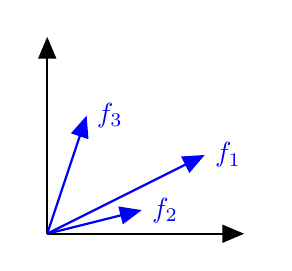
\begin{tikzpicture}[xscale=1,yscale=1,thick]

\draw[->] (0,0) -- (0,2.5) node[left]{$\female$};
\draw[->] (0,0) -- (2.5,0) node[right]{$\male$};

\draw[->,blue] (0,0) -- (2,1) node[right]{$f_1$};
\draw[->,blue] (0,0) -- (1.2,0.3) node[right]{$f_2$};
\draw[->,blue] (0,0) -- (0.5,1.5) node[right]{$f_3$};
\end{tikzpicture}
$$
The first thing to notice is the difference between embedding and meta-embedding: The ideal embedding here is binary, $\zvec\in\{\male,\female\}$, while the meta-embedding is continuous: $f_i\in\R^2$. Here, and in general, the meta-embedding lives in a more complex space than $\zvec$. 

Since likelihoods are positive, the meta-embeddings are confined to the positive quadrant. We should never be working outside of this quadrant, but to see the space as a vector space, we need to be aware of the existence of the other quadrants. Indeed, when we design our neural nets to extract meta-embeddings, we will have to make sure they end up being in the positive quadrant. 

Because of the arbitrary scaling constants, $k_i$, the lengths of our meta-embedding vectors do not carry information---but from the directions we see that $f_1$ and $f_2$ are probably male, while $f_3$ is probably female. Our end-goal is not to infer the genders of the speakers, but to infer whether the speakers of different recordings are the same or not. A little thought should convince the reader that: 
\begin{itemize}
	\item The smallest possible likelihood-ratio, $\frac{P(r_i,r_j\mid H_1)}{P(r_i,r_j\mid H_2)}=0$, would be obtained if we were certain that one speaker is male and the other female. This would happen when we have: 
\begin{align*}
P(r_i\mid\male) &\gg P(r_i\mid\female) &\text{and} && P(r_j\mid\male) &\ll P(r_j\mid\female)
\end{align*}
so that $f_i$ is on the horizontal (male) axis, while $f_j$ is on the vertical (female) axis. Then indeed, the inner product (and dot product) between these two orthogonal meta-embeddings would be zero and so would the LR.
  \item The largest possible LR with the weak, binary hidden variable would be just $2$, which would be obtained when we are certain that both recordings are of the same gender. We need to consider details of the normalization to see how this works out.
\end{itemize}
Figure~\ref{fig:norm} shows the same three meta-embeddings, together with their normalized versions, with normalization as defined by~\eqref{eq:normalize}. Remember the prior-weighting: when $f_i=[f_{i1},f_{i2}]$, then the normalization constant is 
$$\dot{f_i}{\onevec}=\frac12(f_{i1}+f_{i2})$$
Inner products between the normalized meta-embeddings give the likelihood-ratios, 
$$\frac{P(r_i,r_j\mid H_1)}{P(r_i,r_j\mid H_2)}=\dot{\normal{f_i}}{\normal{f_j}}$$ 
Since the discrimination given by the binary hidden variable is weak, the likelihood-ratios are not too far from the neutral value of $1$. The LR, $\dot{\normal{f_1}}{\normal{f_2}}=1.2$ is greater than $1$, slightly favouring the hypothesis that the speakers of $r_1$ and $r_2$ are the same. The other two LRs are less than one, favouring the $H_2$ hypothesis in each case. The LR, $\dot{\normal{f_2}}{\normal{f_3}}=0.64$ is \emph{stronger} (further from $1$) than $\dot{\normal{f_1}}{\normal{f_3}}=0.8$, because we are more certain of the maleness of $f_2$ than we are of $f_1$. The largest possible LR of $2$ would be obtained when both normalized meta-embeddings coincide on the horizontal or vertical axis, at $[2,0]$, or $[0,2]$.\footnote{Remember the prior weighting of $\frac12$.}

%Normalized Meta-Embeddings
\begin{figure}[p]
\centering
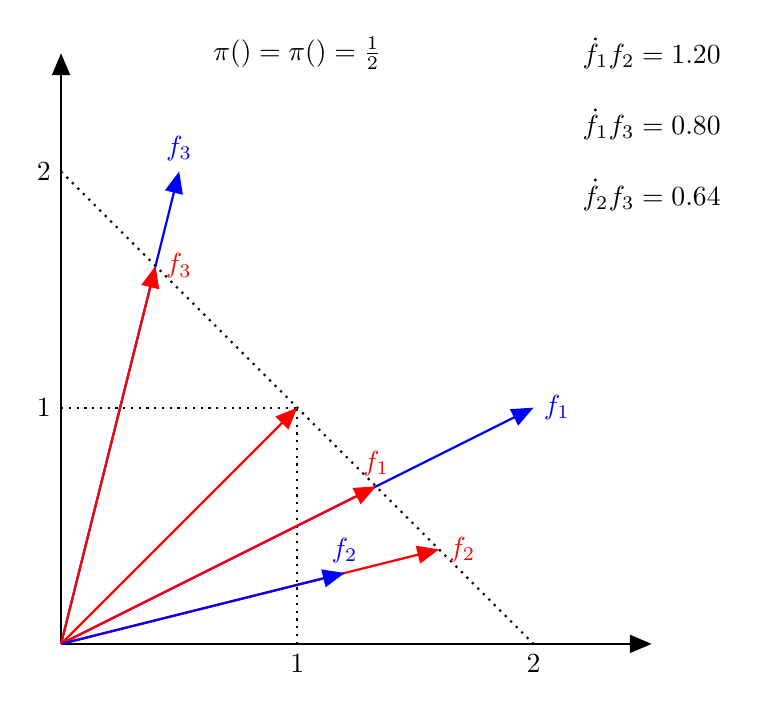
\begin{tikzpicture}[xscale=3,yscale=3,thick]

\draw[->] (0,0) -- (0,2.5) node[left]{$\female$};
\draw[->] (0,0) -- (2.5,0) node[right]{$\male$};
\draw[dotted] (0,2) node[left]{$2$} -- (2,0) node[below]{$2$};

\draw[dotted] (1,0) node[below]{$1$} -- (1,1);
\draw[dotted] (0,1) node[left]{$1$} -- (1,1);
%\node[left] at (0,1) {$1$};
%\node[below] at (1,0) {$1$};
\draw[->,red] (0,0) -- (1,1) node[above right, red]{$\onevec$};

\def\ex{2}\def\ey{1}
\def\fx{1.2}\def\fy{0.3}
\def\gx{0.5}\def\gy{2}

\def\px{{\ex*\fx}}\def\py{{\ey*\fy}}

\def\nex{{2*\ex/(\ex+\ey)}}\def\ney{{2*\ey/(\ex+\ey)}}
\def\nfx{{2*\fx/(\fx+\fy)}}\def\nfy{{2*\fy/(\fx+\fy)}}
\def\ngx{{2*\gx/(\gx+\gy)}}\def\ngy{{2*\gy/(\gx+\gy)}}
\def\npx{{2*\px/(\px+\py)}}\def\npy{{2*\py/(\px+\py)}}

\draw[->,blue] (0,0) -- (\ex,\ey) node[right]{$f_1$};
\draw[->,red] (0,0) -- (\nex,\ney) node[above]{$\normal{f_1}$};

\draw[->,red] (0,0) -- (\nfx,\nfy) node[right]{$\normal{f_2}$};
\draw[->,blue] (0,0) -- (\fx,\fy) node[above]{$f_2$};

\draw[->,blue] (0,0) -- (\gx,\gy) node[above]{$f_3$};
\draw[->,red] (0,0) -- (\ngx,\ngy) node[right]{$\normal{f_3}$};


\node[align=left] at(2.5,2.5){$\dot{\normal{f_1}}{\normal{f_2}}=1.20$};
\node[align=left] at(2.5,2.2){$\dot{\normal{f_1}}{\normal{f_3}}=0.80$};
\node[align=left] at(2.5,1.9){$\dot{\normal{f_2}}{\normal{f_3}}=0.64$};

\node[align=left] at(1,2.5){$\pi(\male)=\pi(\female)=\frac12$};

\end{tikzpicture}  
\caption[Normalized meta-embeddings]{Normalized meta-embeddings (red) and their inner products. Raw meta-embeddings (blue) are normalized by scaling them so that their projections on $\onevec$ are unity.}
\label{fig:norm}
\end{figure}


Figure~\ref{fig:pool} shows what happens when we know that $r_1$ and $r_2$ are of the same speaker and we pool their meta-embeddings, giving us more certainty that this is a male speaker and more certainty that this speaker is different from the (probably female) speaker of $r_3$.



%Pooling
\begin{figure}[p]
\centering
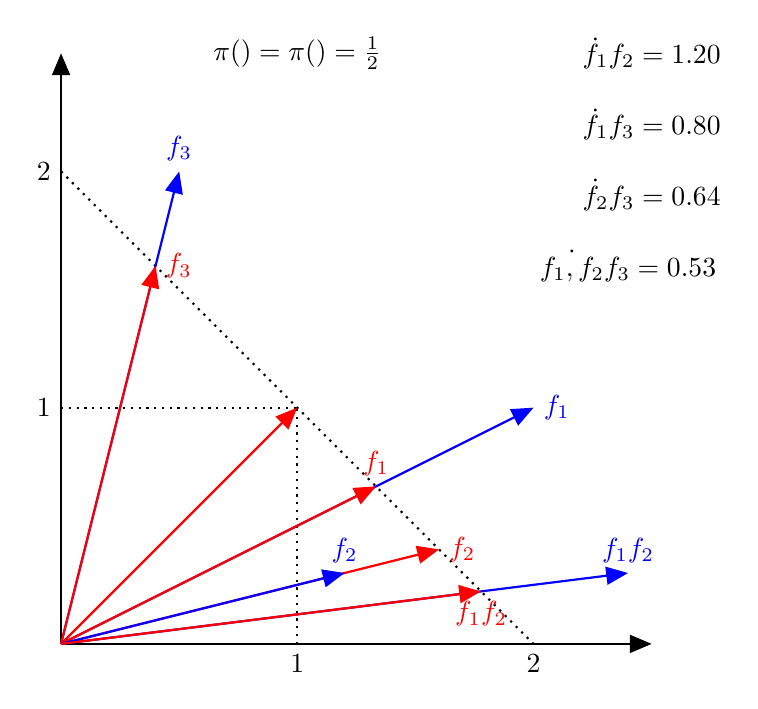
\begin{tikzpicture}[xscale=3,yscale=3,thick]

\draw[->] (0,0) -- (0,2.5) node[left]{$\female$};
\draw[->] (0,0) -- (2.5,0) node[right]{$\male$};
\draw[dotted] (0,2) node[left]{$2$} -- (2,0) node[below]{$2$};
\draw[dotted] (1,0) node[below]{$1$} -- (1,1) node[above right, blue]{$\onevec$};
\draw[dotted] (0,1) node[left]{$1$} -- (1,1);
\draw[->,red] (0,0) -- (1,1) node[above right, red]{$\onevec$};

\def\ex{2}\def\ey{1}
\def\fx{1.2}\def\fy{0.3}
\def\gx{0.5}\def\gy{2}
\def\px{2.4}\def\py{0.3}

\def\nex{{2*\ex/(\ex+\ey)}}\def\ney{{2*\ey/(\ex+\ey)}}
\def\nfx{{2*\fx/(\fx+\fy)}}\def\nfy{{2*\fy/(\fx+\fy)}}
\def\ngx{{2*\gx/(\gx+\gy)}}\def\ngy{{2*\gy/(\gx+\gy)}}
\def\npx{{2*\px/(\px+\py)}}\def\npy{{2*\py/(\px+\py)}}


\draw[->,blue] (0,0) -- (\ex,\ey) node[right]{${f_1}$};
\draw[->,red] (0,0) -- (\nex,\ney) node[above]{$\normal{f_1}$};

\draw[->,red] (0,0) -- (\nfx,\nfy) node[right]{$\normal{f_2}$};
\draw[->,blue] (0,0) -- (\fx,\fy) node[above]{${f_2}$};

\draw[->,blue] (0,0) -- (\gx,\gy) node[above]{${f_3}$};
\draw[->,red] (0,0) -- (\ngx,\ngy) node[right]{$\normal{f_3}$};

\draw[->,blue] (0,0) -- (\px,\py) node[above]{${f_1}{f_2}$};
\draw[->,red] (0,0) -- (\npx,\npy) node[below]{$\normal{{f_1}{f_2}}$};

\node[align=right] at(2.5,2.5){$\dot{\normal{f_1}}{\normal{f_2}}=1.20$};
\node[align=right] at(2.5,2.2){$\dot{\normal{f_1}}{\normal{f_3}}=0.80$};
\node[align=right] at(2.5,1.9){$\dot{\normal{f_2}}{\normal{f_3}}=0.64$};
\node[align=right] at(2.4,1.6){$\dot{\normal{{f_1},{f_2}}}{\normal{f_3}}=0.53$};

\node[align=left] at(1,2.5){$\pi(\male)=\pi(\female)=\frac12$};

\end{tikzpicture}
\caption[Meta-embedding pooling]{Pooling: If we know that $f_1$ and $f_2$ are from the same speaker, we can pool them, using the elementwise product $f_1f_2$. This increases the certainty that this is a male speaker. Correspondingly, the strength (difference from $1$) of $\dot{\normal{f_1f_2}}{\normal{f_3}}$ is more than either of $\dot{\normal{f_1}}{\normal{f_3}}$ and $\dot{\normal{f_2}}{\normal{f_3}}$. Pooling has increased the certainty that the speaker represented by $f_1f_2$ is not the same speaker as the probably female $f_3$.}
\label{fig:pool}
\end{figure}




\chapter{Practical meta-embeddings}
We have thus far developed a theoretical idea of the nature of meta-embeddings. We are now ready to explore a few proposals of how to practically represent meta-embeddings. The end-goal is to train a neural net that takes voice recordings as input and outputs  representations for the corresponding meta-embeddings. We shall discuss training criteria for the neural net later. Here we are interested in the form that practical meta-embedding representations might take and we shall explore several possibilities. \\

\noindent Before proceeding to these possibilities, let us consider in general, some desirable properties of our representations. Ideally, we need all of the following properties for our meta-embeddings:
\begin{itemize}
	\item[] \textbf{Non-negativity:} $f(\zvec)\ge0$ everywhere.
	\item[] \textbf{Normalizability:} $\dot{f}{\onevec}<\infty$.
	\item[] \textbf{Pooling} should be tractable, and the pooled result, $f_if_j$, should have the same representation as $f_i$ and $f_j$.
	\item[] \textbf{Expectation:}  $\expv{f(\zvec)}{\zvec\sim\pi}$ should be tractable for any meta-embedding $f$, whether it is raw or pooled.
	\item[] \textbf{Backpropagation} of derivatives through pooling and expectation is necessary for training.
\end{itemize}
Recall that if we can pool and do expectations, then we can also do any inner products, since $\dot{f}{g}=\expv{fg}{}$.

The first two proposals below, based on exponential family distributions, meet all of these requirements, although the expectations are somewhat computationally expensive. In some of the other proposals, various approximations and compromises have to be made.



\section{Multivariate Gaussian}
\label{sec:MVG}
\def\dvec{\mathbf{d}}
This recipe supposes a continuous speaker identity variable, $\zvec\in\R^d$. A trainable neural net processes each recording, $r_j$, and outputs the corresponding meta-embedding, $f_j$, in the form of a $(d+D)$-dimensional representation:
$$r_j\mapsto\evec_j=(\avec_j,\bvec_j)$$
where $\avec\in\R^d$ and $\bvec_j=(b_{1j},\ldots,b_{Dj})\in\R_+^D$, where $D\ge1$ and the $b_{ij}\ge0$. While the representation, $\evec_j$, is finite-dimensional, it parametrizes the \emph{infinite-dimensional} meta-embedding, $f_j$, defined as:
\begin{align}
\label{eq:gaussembed}
f_j(\zvec) &= \exp\bigl[\avec_j'\zvec -\frac12\zvec'\Bmat_j\zvec]
\end{align}
where $\Bmat_j$ is a $d$-by-$d$, positive semi-definite precision matrix, composed as a conical combination:
\begin{align}
\label{eq:Bmat}
\Bmat_j &= \sum_{i=1}^D b_{ij} \Emat_i
\end{align}
where $\{\Emat_i\}_{i=1}^D$ are fixed, $d$-by-$d$, positive semi-definite definite matrices---they are fixed in the sense of being independent of the input data (recordings), but the elements of these matrices are still trainable, together with the parameters of the neural net that extracts the $\evec_j$. These matrices can be full, low rank, diagonal, etc. 

Since $\zvec\in\R^d$ is hidden, we are free to choose the dimensionality, $d$. Experience with PLDA suggests $100\le d\le200$ is a good choice. This can also be compared to the Facenet embeddings, which are 120-dimensional. The size, $D$, of the precision parametrization can be used to trade off computational complexity vs capacity. To keep the complexity significantly less than that which would be needed for fully specified precision matrices, we probably want to constrain $D\ll\frac{d(d+1)}{2}$. 

Scalar multiplication could be easily done in this framework but in practice, we probably won't need it. Addition of the meta-embeddings would give mixtures of Gaussians, with more complex representations, but for this representation we don't need addition.

\subsection{Elementwise product}
The important elementwise product is done by simply adding the representation vectors. For $\Rset=\{r_1,\ldots,r_n\}$, we can extract the individual representations, $\{\evec_j\}_{j=1}^n$, which respectively represent the $\{f_j\}_{j=1}^n$. The representation for $f_\Rset=\prod_{j=1}^n f_j$ is then $\evec_\Rset=\sum_{j=1}^n \evec_j$. The representation $\evec_j$ is essentially logarithmic, which gives us the benefit of automatic positivity, as well as easy elementwise multiplication. The disadvantage is somewhat complex expectation computation.


\subsubsection{Note on group structure}
For future reference, it might be useful to note that since Gaussians are closed under (associative) multiplication, our space of Gaussian meta-embeddings is a \emph{monoid} (a semigroup, with identity). Since we exclude precision matrices with negative eigenvalues, our monoid lacks inverse elements, which would have made it a full group. The identity element is a Gaussian with zero mean and zero precision, which is just our previously defined identity, $\onevec(\zvec)=1$. 


\subsection{Prior}
To do expectations we need to define the prior. The simplest choice is the standard Gaussian:\footnote{Note here and elsewhere, we use two different fonts to differentiate $\pi(\zvec)$, from the trigonometric constant $\uppi$.}
\begin{align}
\pi(\zvec) &= \ND(\zvec\mid\nulvec,\Imat) = \frac{e^{-\frac12\zvec'\zvec}}{\sqrt{(2\uppi)^d}}
\end{align}

\subsection{Expectation}
Since our logarithmic representation is closed under elementwise multiplication, our expectations can always be performed on representations of the form~\eqref{eq:gaussembed}. Dropping the subscript $j$ to avoid clutter, we derive an expression for $E(\avec,\Bmat)=\expv{f}{}$, where $f(\zvec)=\exp[\avec'\zvec-\frac12\zvec'\Bmat\zvec]$:
\begin{align}
\label{eq:MVGproblem}
\begin{split}
E(\avec,\Bmat) &= \expv{f}{} \\
&= \int_{\R^d} f(\zvec)\pi(\zvec) \,d\zvec \\
&= \int_{\R^d} f(\zvec)\ND(\zvec\mid\nulvec,\Imat) \,d\zvec \\
&= \int_{\R^d} \frac{\exp\bigl[\avec'\zvec -\frac12\zvec'(\Imat+\Bmat)\zvec\bigr]}{\sqrt{(2\uppi)^d}} \,d\zvec 
\end{split}
\end{align}
If we define $\muvec=(\Imat+\Bmat)^{-1}\avec$, we can rewrite this as:
\begin{align}
\label{eq:exactMVG}
\begin{split}
E(\avec,\Bmat) &= \expv{f}{} \\
&= \int_{\R^d} \frac{\exp\bigl[\muvec'(\Imat+\Bmat)\zvec -\frac12\zvec'(\Imat+\Bmat)\zvec\bigr]}{\sqrt{(2\uppi)^d}} \,d\zvec \\
&= \frac{\exp\bigl[\frac12\muvec'(\Imat+\Bmat)\muvec\bigr]}{\abs{\Imat+\Bmat}^{\frac12}}
\int_{\R^d} \frac{\abs{\Imat+\Bmat}^\frac12}{\sqrt{(2\uppi)^d}} \exp\bigl[-\frac12(\zvec-\muvec)'(\Imat+\Bmat)(\zvec-\muvec)\bigr]\,d\zvec \\
&= \frac{\exp\bigl[\frac12\muvec'(\Imat+\Bmat)\muvec\bigr]}{\abs{\Imat+\Bmat}^{\frac12}} \int_{\R^d} \ND(\zvec\mid\muvec,(\Imat+\Bmat)^{-1}) \,d\zvec \\
&= \frac{\exp\bigl[\frac12\muvec'(\Imat+\Bmat)\muvec\bigr]}{\abs{\Imat+\Bmat}^{\frac12}} \\
&= \frac{\exp\bigl[\frac12\avec'\muvec\bigr]}{\abs{\Imat+\Bmat}^{\frac12}} 
\end{split}
\end{align}
Both $\muvec$ and the determinant $\abs{\Imat+\Bmat}$ can be found by Cholesky decomposition of the positive definite matrix $\Imat+\Bmat$.

%\subsubsection{Backpropagation}
%Derivation of the backpropagating equations for $E(\avec,\Bmat)$ can be done by using the fact that the derivatives w.r.t.\ the natural parameters of the log-normalizer of any exponential family distribution give the expected values of the sufficient statistics.


%\subsection{Expectation via maximization}
%We want to find the value of integral~\eqref{eq:MVGproblem}:
%\begin{align}
%\begin{split}
%E(\avec,\Bmat) &= \int_{\R^d} \frac{\exp\bigl[\avec'\zvec -\frac12\zvec'(\Imat+\Bmat)\zvec\bigr]}{\sqrt{(2\uppi)^d}} \,d\zvec  \\
%&= 
%\end{split}
%\end{align}

\subsubsection{The one-dimensional case}
To better understand this formula, let us examine the one-dimensional case, $\Zset=\R$. Denoting $b=\Bmat$ and $a=\avec$, where $a\in\R$ and $b\ge0$, we find:
\begin{align}
\begin{split}
E(a,b) &= \frac{e^{\frac12\frac{a^2}{1+b}}}{\sqrt{1+b}} \\
&= \frac1{\sqrt{2\uppi}(1+b)\ND(a\mid0,1+b)}\\
&= \frac1{1+b}\,\frac{\ND(0\mid0,1)}{\ND(0\mid a,1+b)}\\
\end{split}
\end{align}
Given two meta-embeddings, $f_1,f_2$, respectively represented by $(a_1,b_1)$ and $(a_2,b_2)$, the LR between them is:
\begin{align}
\begin{split}
\dotn{f_1}{f_2} &= \frac{E(a_1+a_2,b_1+b_2)}{E(a_1,b_1)E(a_2,b_2)} \\
&= \frac{(1+b_1)(1+b_2)}{1+b_1+b_2}\,\frac{\ND(0\mid a_1,1+b_1)\ND(0\mid a_2,1+b_2)}{\ND(0\mid 0,1)\ND(0\mid a_1+a_2,1+b_1+b_2)}
\end{split}
\end{align} 


\subsection{Examples}
Let us again turn to some simple examples to better understand our multivariate Gaussian meta-embeddings. We choose $\zvec\in\Zset=R^2$, so that we can plot the examples. Recall that in the example of section~\ref{sec:exem} we were able to directly plot points in meta-embedding space. Here, that space is infinite-dimensional, so we cannot plot our meta-embeddings as points. But we \emph{can} plot representations of the Gaussian \emph{distributions} in $\Zset$-space. 

In our plots below, every meta-embedding is shown as an ellipse, centered at the mean of the Gaussian. The ellipse represents the $\sigma=1$ contour so that it is elongated in directions where the meta-embedding has less certainty about the location of $\zvec$, while the ellipse is more compressed in directions of greater certainty.\footnote{The ellipse axes are aligned with the eigenvectors of the covariance, and the radii are the square roots of the eigenvalues. MATLAB code that computes LLRs and outputs Ti\emph{k}Z code for plotting the ellipses in \LaTeX~is available here: \url{http://github.com/bsxfan/meta-embeddings/tree/master/code/Niko/matlab}.}

The figure below shows some hypothetical meta-embeddings and the LRs between them, computed using~\eqref{eq:exactMVG} in~\eqref{eq:slrdot}, or \eqref{eq:mlrdot}. The standard normal prior is shown in dashed black. Blue, red and green represent raw embeddings, while magenta represents blue and red pooled, where pooling is done by adding natural parameters ($\avec_\text{mag} = \avec_\text{blue} + \avec_\text{red}$, and $\Bmat_\text{mag} = \Bmat_\text{blue} + \Bmat_\text{red}$):  
$$
\begin{tikzpicture}[xscale=1.5,yscale=1.5]
\draw[rotate around ={   0:(   0,   0)},black, dashed] (   0,   0) ellipse [x radius=   1, y radius=   1];
\draw[rotate around ={  45:(-0.7,   0)},blue] (-0.7,   0) ellipse [x radius=0.632, y radius=0.707];
\draw[rotate around ={  90:(  -1,   0)},red] (  -1,   0) ellipse [x radius=0.316, y radius=   1];
\draw[rotate around ={   0:(   1,   0)},green] (   1,   0) ellipse [x radius=0.408, y radius=0.408];
\draw[rotate around ={88.4:(-0.792,0.00189)},magenta] (-0.792,0.00189) ellipse [x radius=0.286, y radius=0.555];
%
\node[ctext] at(4,0) {%
\begin{tabular}{c|rrr}
$\dotn{f_i}{f_j}$ & blue & red & magenta \\
\hline
green & 0.37  & 0.80 & 0.23 \\
blue & & 2.34 &  
\end{tabular}%
};
\end{tikzpicture}
$$
We can imagine that green was extracted from a long, clean recording; blue from a long noisy recording; and red from a short, clean recording. The short red recording gives reasonable certainty along the vertical axis, but crucial information is missing, resulting in greater uncertainty on the horizontal axis. Notice that $\LRT{blue}{green}<\LRT{red}{green}$, even though the blue mean is closer to green than the red mean. This is due to the greater red uncertainty in the horizontal direction. Pooling (magenta) dramatically reduces the uncertainty about the location of $\zvec$ for the speaker represented by red and blue and consequently increases the certainty that this speaker is \emph{not} the same as the green speaker: $\LRT{magenta}{green}$ is smaller than all the other LRs. There is enough overlap between red and blue to give some support, $\LRT{red}{blue}>1$, for the hypothesis that red and blue are of the same speaker. 

Next, we repeat the example, keeping everything the same, except that all the embeddings have smaller uncertainty. The effect is that the LRs also become more certain, moving further away from the neutral value of 1: 
$$
\begin{tikzpicture}[xscale=1.5,yscale=1.5]
\draw[rotate around ={   0:(   0,   0)},black, dashed] (   0,   0) ellipse [x radius=   1, y radius=   1];
\draw[rotate around ={  45:(-0.7,   0)},blue] (-0.7,   0) ellipse [x radius=0.365, y radius=0.408];
\draw[rotate around ={  90:(  -1,   0)},red] (  -1,   0) ellipse [x radius=0.183, y radius=0.577];
\draw[rotate around ={   0:(   1,   0)},green] (   1,   0) ellipse [x radius=0.236, y radius=0.236];
\draw[rotate around ={88.4:(-0.792,0.00189)},magenta] (-0.792,0.00189) ellipse [x radius=0.165, y radius=0.321];
%
\node[ctext] at(3.5,0) {%
\begin{tabular}{c|rrr}
$\dotn{f_i}{f_j}$ & blue & red & magenta \\
\hline
green & 0.008  & 0.069 & 7.4e-4 \\
blue & & 5.264 &  
\end{tabular}%
};
\end{tikzpicture}
$$
Finally, we change the example by shifting the meta-embeddings left, relative to the prior. This affects all the LRs:
$$
\begin{tikzpicture}[xscale=1.5,yscale=1.5]
\draw[rotate around ={   0:(   0,   0)},black, dashed] (   0,   0) ellipse [x radius=   1, y radius=   1];
\draw[rotate around ={  45:(-1.7,   0)},blue] (-1.7,   0) ellipse [x radius=0.365, y radius=0.408];
\draw[rotate around ={  90:(  -2,   0)},red] (  -2,   0) ellipse [x radius=0.183, y radius=0.577];
\draw[rotate around ={   0:(   0,   0)},green] (   0,   0) ellipse [x radius=0.236, y radius=0.236];
\draw[rotate around ={88.4:(-1.79,0.00189)},magenta] (-1.79,0.00189) ellipse [x radius=0.165, y radius=0.321];
\node[ctext] at(3.5,0) {%
\begin{tabular}{c|rrr}
$\dotn{f_i}{f_j}$ & blue & red & magenta \\
\hline
green & 0.015  & 0.162 & 0.0013 \\
blue & & 14.260 &  
\end{tabular}%
};
\end{tikzpicture}
$$
The most dramatic effect of the above shift is on $\LRT{red}{blue}$, which has increased threefold due to the increased rarity of the red and blue embeddings, relative to the prior.


\subsubsection{Food for thought}
Let us examine pooling in more detail. In the above examples, when we pooled the suboptimal information extracted by the (short) red and (noisy) blue recordings, the result (magenta) gave less uncertainty about the value of $\zvec$ for the speaker common to red and blue. Intuition suggests that things are working properly. But now consider pooling red and blue embeddings which are far apart:
$$
\begin{tikzpicture}[xscale=1,yscale=1]
%\draw[rotate around ={   0:(   0,   0)},black, dashed] (   0,   0) ellipse [x radius=   1, y radius=   1];
\draw[rotate around ={  45:(  -2,   0)},blue] (  -2,   0) ellipse [x radius=0.707, y radius=0.392];
\draw[rotate around ={  45:(   2,2.96e-016)},red] (   2,2.96e-016) ellipse [x radius=0.577, y radius=   1];
\draw[rotate around ={  45:(-0.533,0.933)},magenta] (-0.533,0.933) ellipse [x radius=0.447, y radius=0.365];
%\draw[rotate around ={  45:(-2.22e-016,2.96e-016)},green] (-2.22e-016,2.96e-016) ellipse [x radius=0.913, y radius=1.07];
%
\node[ctext] at(6,0) {%
$\LRT{blue}{red}=0.0047$
};
\end{tikzpicture}
$$
This result (magenta) is perhaps counter-intuitive: 
\begin{itemize}
	\item Why is the magenta mean so far away from the line connecting the red and blue means? 
	\item If the same speaker is observed in two relatively distant locations, should this not cause the resulting uncertainty to \emph{increase}, rather than the decrease we see here?
\end{itemize}
Nevertheless, we have followed the theory and the magenta result is correct. One reason why our intuition has a hard time to accept this result is because pooling is conditioned on the assumption that the speakers are the same, yet $\LRT{blue}{red}\ll 1$ gives strong support to the hypothesis that blue and red are in fact different speakers. If we were to encounter this situation in practice, it would suggest that the same-speaker assumption is wrong, or that the uncertainties in the meta-embeddings have been underestimated.

The apparently wayward magenta mean is the location where the blue and red distributions `overlap most'. It is located at the maximum of the product of the two distributions. It can be interpreted as a soft intersection between the two distributions.

\subsection{Stochastic expectation}
\def\tvec{\mathbf{t}}
Pooling is fast (addition) but expectation is slower (Cholesky decomposition). Unfortunately, our recipe above requires a new Cholesky decomposition for every LR calculation. In applications where many verification trials are processed on limited hardware, this will have a significant impact on speed. Even if we have enough CPU power available at runtime for some applications, training remains a problem because we are going to be training our meta-embedding extractors with discriminative criteria that typically require evaluating very many trials. Let us therefore consider some plans for speeding up scoring of trials by making stochastic approximations.

We envisage that such stochastic approximation could work out to be especially cheap at training time, in the same way that stochastic evaluation of the ELBO in \emph{variational autoencoder} (VAE) training typically requires but a single stochastic sample per training example~\cite{VAE}. Given sufficiently many examples, the stochastic approximation errors tend to cancel, provided the errors are independent. 

We will not be too concerned about expectations of a single factor, of the form $\expv{f}{}$. These expectations are required to normalize trial sides (typically meta-embeddings extracted from single recordings) and there are far fewer trial sides than there are trials. The calculations for which we need speed, are expectations of the form $\expv{\normal{f_i}\,\normal{f_j}}{}$. We consider three solutions below.\\

\subsubsection{Prior sampling}
An obvious choice, perhaps naive, would be to form the expectation by sampling from the prior, $\pi$. The expectation could be approximated via $m$ such samples as:
\begin{align}
\expv{\normal{f_i}(\zvec)\normal{f_j}(\zvec)}{\zvec\sim\pi} &\approx \frac1m\sum_{\tilde\zvec\sim\ND(\nulvec,\Imat)} \normal{f_i}(\tilde \zvec)\normal{f_j}(\tilde \zvec)
\end{align}
We fear this might be inaccurate, because in high-dimensional space, samples from $\pi$ will be very unlikely to hit the peak\footnote{The product is still Gaussian and therefore has single peak.} of $\normal{f_i}\,\normal{f_j}$ and therefore an affordable number of samples might not be able to sufficiently explore the volume under the peak. Experiments might be needed to check whether this is indeed a problem. Let us nevertheless explore in more detail the calculation required for each sample:
\begin{align}
\label{eq:priorsampling}
\begin{split}
\normal{f_i}(\tilde \zvec)\normal{f_j}(\tilde \zvec) 
&= c_ic_j\exp\bigl[
\avec'_i\tilde\zvec +\avec_j'\tilde\zvec -\frac12\tilde\zvec'\Bmat_i\tilde\zvec  -\frac12\tilde\zvec'\Bmat_j\tilde\zvec
\bigr]\\
&= c_ic_j\exp\bigl[
\avec'_i\tilde\zvec +\avec_j'\tilde\zvec -\frac12 \bvec'_i\tilde\gammavec -\frac12 \bvec'_j\tilde\gammavec
\bigr]\\
\end{split}
\end{align}
where using~\eqref{eq:Bmat}, we have defined $\tilde\gammavec = [\tilde\gamma_1,\ldots,\tilde\gamma_D]\in\R^D$, with $\tilde\gamma_\ell = \tilde\zvec'\Emat_\ell\tilde\zvec$ and 
where $c_i,c_j$ reflect the normalizations. The meta-embedding representations, $\avec_i,\bvec_i$ and $\avec_j,\bvec_j$, and the trainable constants, $\{\Emat_\ell\}_{\ell=1}^D$, are as defined in the beginning of section~\ref{sec:MVG}. 

Notice that $\tilde\gammavec$ is independent of the meta-embeddings and therefore independent of the data and can be precomputed. If the $\Emat_\ell$ are constrained to be either diagonal or rank-one, then the calculations $\tilde\zvec'\Emat_\ell\zvec$ will be cheap. Keep in mind that we need $m$ different samples, $\tilde\zvec$, and therefore also $m$ different versions of $\tilde\gammavec$. In stochastic minibatch training, if we update the $\{\Emat_\ell\}$ after every minibatch, we will have to update all of the $\tilde\gammavec$ also, in which case it might make sense to also resample $m$ new values for $\tilde\zvec$. This type of strategy, which is well-known also in VAE~\cite{VAE}, is termed \emph{doubly stochastic} by Michalis Titsias~\cite{Titsias}. 

An advantage of~\eqref{eq:priorsampling} is that it generalizes to expectations of more (or fewer) than two factors---the argument in the exponent will have independent terms for each of the factors in the expectation.

Experiments would have to be conducted to verify if an affordably small $m$ could give reasonable accuracy. Keep in mind that in such experiments, we can compare accuracy against the exact calculation~\eqref{eq:exactMVG}.\\

%\subsubsection{Transformed prior sampling}
%\begin{align}
%\begin{split}
%&\int_{\R^n} \pi(\zvec) \frac{\ND(\zvec\mid\Bmat^{-1}\avec,\Bmat^{-1})}{\sqrt{\detm{\Bmat}}}  \,d\zvec  \\
%&= \frac1{(2\uppi)^d} \int_{\R^n} \CT{\pi}(\tvec)\, \frac{\CT{\ND(\Bmat^{-1}\avec,\Bmat^{-1})}(\tvec)}{\sqrt{\detm{\Bmat}}}  \,d\tvec  \\
%&= \frac1{(2\uppi)^d} \int_{\R^n} \sqrt{\detm{2\uppi\Imat}}\pi(\tvec) \, \frac{\sqrt{\detm{2\uppi\Bmat}}\cos(\tvec'\Bmat^{-1}\avec)\ND(\tvec\mid\nulvec,\Bmat)}{\sqrt{\detm{\Bmat}}}  \,d\tvec  \\ 
%&= \int_{\R^n} \pi(\tvec) \, \cos(\tvec'\Bmat^{-1}\avec)\ND(\tvec\mid\nulvec,\Bmat)  \,d\tvec  
%\end{split}
%\end{align}


\subsubsection{Posterior sampling} 
If meta-embedding $f_i$ represents recording $r_i$, then $$\pi(\zvec)\normal{f_i}(\zvec)=P(\zvec\mid r_i,\pi)$$ is a properly normalized Gaussian, from which we can sample.\footnote{The same is not always true of $f_i$ or $\normal{f_i}$, which might have a singular precision, in which case sampling could not be done.} We can now rewrite the expectation as:
\begin{align}
\expv{\normal{f_i}(\zvec)\normal{f_j}(\zvec)}{\zvec\sim\pi} &= \expv{\normal{f_j}(\tilde\zvec)}{\tilde\zvec\sim\pi\normal{f_i}}
\approx\frac1m\sum_{\tilde\zvec\sim\pi\normal{f_i}}c_j\exp\bigl[\avec'_j\tilde\zvec -\frac12\bvec'_j\tilde\gammavec\bigr]
\end{align}
This might be more accurate than prior sampling, because when $f_i$ and $f_j$ represent the same speaker, their peaks should overlap. If they are of different speakers, their peaks might be far apart, but then we do want a value close to zero for the expectation. With this variant, we may be able to use smaller values for $m$. 

This method is asymmetric. Which version is best---should we sample from $f_i$, or from $f_j$? If $f_i$ is much sharper than $f_j$, so that $f_j$ is almost constant compared to $f_j$, then one sample would suffice, while if we sampled the other way round, we would need many samples to properly explore the volume of $f_i$. Pooling generally sharpens peaks, so it would be more accurate to sample from the side that consists of the most pooled factors. Unfortunately, fast pooling and sampling are conflicting requirements---after adding natural parameters to compute the pooling, we need a Cholesky factorization before we can sample.

Whether we pool or not, a disadvantage of posterior sampling vs prior sampling is that we have reintroduced the need for Cholesky factorization. Fortunately, we need this only for one side of the trial and we are still avoiding per-trial Cholesky decompositions. Also note that for the sampled side of the trial we do not need to separately compute the normalization constant, because the samples already come from the normalized distribution. 

Another option would be to change the representation. We could let:
\begin{align}
\Bmat_i &= \Bigl(\sum_{\ell=1}^D b_{\ell i} \Tmat_\ell \Bigr)\Bigl(\sum_{\ell=1}^D b_{\ell i} \Tmat_\ell \Bigr)'
\end{align}  
where the $\Tmat_\ell$ are triangular and the $b_{\ell i}$ are no longer constrained to be non-negative. This gives a free Cholesky decomposition, and fast, approximate evaluation of LRs of the form $\dot{\normal{f_i}}{\normal{f_j}}$, but it complicates pooling for more complex LR calculations.\\


\section{Zero-mean Gaussians}
Next, let us place a restriction on our multivariate Gaussian embeddings in the quest for fast and accurate stochastic expectation solutions. By restricting meta-embeddings to \emph{zero-mean Gaussians with strictly positive definite precisions}, the Fourier transforms of these Gaussians always exist and are also multivariate Gaussians---from which we can sample in the frequency domain. By Parseval's theorem, we can compute the expectation integrals instead in the frequency domain. By the convolution theorem, products of Gaussians in the original $\Zset$ domain become convolutions in the frequency domain. These convolutions can be stochastically implemented by \emph{adding} samples drawn from individual meta-embeddings. We now have made both pooling and expectation \emph{simultaneously easy}---a property which has thus far eluded us. The disadvantage is that we have lost the capacity for the meta-embeddings to have means and it is not immediately obvious whether this would be a serious drawback for the application at hand. 

Before continuing to the details below, we recommend that the reader review appendix~\ref{chap:MDFT} on multidimensional Fourier transforms and characteristic functions. Characteristic functions and Fourier transforms of probability densities are equivalent up to linear reparametrization. For our application, it will be more convenient to work with characteristic functions.

\subsection{Representation}
For this representation, we have already restricted our meta-embeddings to zero-mean normal distributions. The normalization constants of these distributions are irrelevant, for the same reason that we have allowed all our meta-embeddings to have arbitrary scale factors. As shown in the appendix~\ref{sec:GCF}, for meta-embedding $f_i(\zvec)\propto\ND(\zvec\mid\nulvec,\Bmat_i^{-1})$, the characteristic function is:
\begin{align}
\CT{f_i}(\tvec) = \phi_i(\tvec) = k_i\,\ND(\tvec\mid\nulvec,\Bmat_i)
\end{align} 
where $k_i$ is a scaling constant. The prior, $\pi(\zvec)=\ND(\zvec\mid\nulvec,\Imat)$, transforms as:
\begin{align}
\CT{\pi}(\tvec) = \phi_0(\tvec) = (2\uppi)^{d/2} \ND(\tvec\mid\nulvec,\Imat) = k_0\pi(\tvec)
\end{align} 
Since there is a bijection between densities and characteristic functions, we may as well directly extract representations for the $\phi_i$. Moreover, these representations can be conveniently chosen to facilitate sampling. That is, every $\phi_i$ is represented by a $d$-by-$d$ square (possibly triangular) matrix. Sampling is done by forming matrix vector products, where the $d$-dimensional vectors are sampled from the standard Gaussian. This is just the \emph{reparametrization trick}, familiar from the VAE literature, which plays well with gradient backpropagation through the stochastic part of the calculation~\cite{VAE}. 

More parsimonious representations are possible. We can represent each meta-embedding via \emph{samples}, rather than via a matrix of parameters. The net that extracts the embeddings is simply required to produce Gaussian samples, using any convenient method. One way to implement this is to generate samples from a factor analysis model---where samples drawn from a full rank diagonal Gaussian are added to $D$-dimensional samples multiplied by a $D$-by-$d$ factor loading matrix, where typically $D\ll d$. The parameter count of the factor-analysis representation  is $d(D+1)$, compared to $d^2$ for full, or $\frac{d(d+1)}{2}$ for triangular covariance square-root parametrizations.

\subsection{Frequency domain pooling and expectation}
We are interested in expectations of the form $\expv{\prod_{i=1}^m f_i}{\pi}$, which we rewrite via Parseval (\ref{sec:cfParseval}) and the convolution theorem (\ref{sec:cfConvolution}) as:
\begin{align}
\begin{split}
\int_{\R^n} \pi(\zvec) \prod_{i=1}^m f_i(\zvec)  \,d\zvec  
&= \frac{1}{(2\uppi)^d}\int_{\R^n} \CT{\pi}(\tvec) \CT{f_1\cdots f_m}(\tvec) \,d\tvec  \\
&= \frac{k_0}{(2\uppi)^d}\int_{\R^n} \pi(\tvec) \CT{f_1\cdots f_m}(\tvec) \,d\tvec  \\
&= \frac{k_0}{(2\uppi)^d}\int_{\R^n} \pi(\tvec) \CT{f_1}\ast\cdots\ast\CT{f_m}(\tvec) \,d\tvec  \\
&= \frac{k_0k_1\cdots k_m}{(2\uppi)^d}\int_{\R^n} \pi(\tvec) \ND(\tvec\mid\nulvec,\Bmat_1)\ast\cdots\ast\ND(\tvec\mid\nulvec,\Bmat_m) \,d\tvec  \\
&= \frac{k_0k_1\cdots k_m}{(2\uppi)^d}\int_{\R^n} \pi(\tvec) \ND\bigl(\tvec\mid\nulvec,\sum_{i=1}^m\Bmat_i\bigr) \,d\tvec  \\
\end{split}
\end{align}
where $\ast$ denotes convolution and where we do not need complex conjugation, because everything is real-valued. Since $\pi$ is standard Gaussian, its Fourier transform is also standard Gaussian. The RHS is the expected value of $\pi$, w.r.t.\ a Gaussian, formed by the convolution of $m$ zero-mean Gaussians, $\{\tilde f_i\}$. The sum of independent samples of all the $\tilde f_i$ will give a sample from the convolution. These sums can then be inserted into $\pi$ and averaged to approximate the required expectation.

\subsection{Could it work?}
The question is whether meta-embeddings without means could distinguish between speakers. All our meta-embeddings share the same expected value. All peaks coincide. Still, these concentric Gaussians can be very different, with probability mass spread in different directions in $\R^d$ space. 

\subsection{Complex Gaussians}
Do complex Gaussians perhaps have complex Gaussians as Fourier transforms? Can we get around the zero-mean restriction in this way? 



\section{Exponential family Gaussian mixture}
The multivariate Gaussian of the previous section is of course an exponential family distribution. We can derive very similar recipes---also with logarithmic representations---from other exponential families. We develop one such example here.

Although a Gaussian mixture is not an exponential family, the \emph{joint} distribution for the continuous and discrete (state) variable \emph{is} exponential family. We do this with a $D$-component mixture of $d$-dimensional Gaussians, by choosing our hidden speaker identity variable as: $\zvec=(\xvec,\yvec)$, where $\xvec=(x_1,\ldots,x_D)$ is a one-hot vector of size $D$, while $\yvec\in\R^d$. Our meta-embedding for recording $j$ is:
\begin{align}
f_j(\xvec,\yvec) &= \prod_{i=1}^D \Bigl(w_{ij}\exp\bigl[\avec'_{ij}\yvec-\frac12\yvec'\Bmat_{ij}\yvec\bigr]\Bigr)^{x_i}
\end{align}
where $x_i\in\{0,1\}$, $w_{ij}>0$, $\avec_{ij}\in\R^d$ and the $\Bmat_{ij}$ are $d$-by-$d$ positive semi-definite. To see that this is exponential family, take the logarithm and re-arrange:
\begin{align}
\log f_j(\xvec,\yvec) &= \sum_{i=1}^D x_i\log w_{ij} + (x_i\yvec')\avec_{ij}-\frac12\trace\bigl[(x_i\yvec\yvec')\Bmat_{ij}\bigr]
\end{align}
where we see the sufficient statistics are: $\{x_i,x_i\yvec,x_i\yvec\yvec'\}_{i=1}^D$ and the natural parameters are $\{\log w_{ij},\avec_{ij},\Bmat_{ij}\}_{i=1}^D$. To form more compact representations, we can let the natural parameters be linear functions of smaller vectors (of which some components have to be constrained to be non-negative). As above, elementwise multiplication (pooling) is accomplished by simple vector addition of these representations. 

\subsection{Prior}
We choose a parameterless prior, of the same form as the meta-embeddings:
\begin{align}
\pi(\xvec,\yvec) &= \prod_{i=1}^D \Bigl(\frac{\ND(\yvec\mid\nulvec,\Imat)}{D}\Bigr)^{x_i}
\end{align} 
and
\begin{align}
\begin{split}
\log \pi(\xvec,\yvec) &= \sum_{i=1}^D x_i \bigl( -\frac12\yvec'\yvec -\frac{d}{2}\log(2\uppi) -\log(D)\bigr) \\
&= -\frac{d}{2}\log(2\uppi) -\log(D) + \sum_{i=1}^D -\frac12\trace\bigl[(x_i\yvec\yvec')\Imat\bigr]
\end{split}
\end{align}
As in the multivariate Gaussian case, the practical function of the prior is to add $\Imat$ to the possibly semi-definite matrices, $\Bmat_{ij}$, of the meta-embeddings, to make them properly positive definite. 


\subsection{Expectation}
\def\Oset{\mathcal{O}}
Dropping the subscript $j$, let $f(\xvec,\yvec) = \prod_{i=1}^D \Bigl(w_i\exp\bigl[\avec'_i\yvec-\frac12\yvec'\Bmat_i\yvec\bigr]\Bigr)^{x_i}$, then:\footnote{We abuse notation by writing $\xvec=i$ to indicate that component $i$ is the hot element (value 1) in the otherwise zero one-hot vector, $\xvec$.}
\begin{align}
\begin{split}
E\bigl(\{w_i,\avec_i,\Bmat_i\}_{i=1}^D\bigr) &= \expv{f}{} \\
&= \sum_{i=1}^D \frac{w_i}{D} \int_{\R^d} f(\xvec=i,\yvec) \ND(\yvec\mid\nulvec,\Imat)\;d\yvec  \\
&= \sum_{i=1}^D \frac{w_i}{D} \int_{\R^d} \exp\bigl[\avec'_i\yvec-\frac12\yvec'\Bmat_i\yvec\bigr] \ND(\yvec\mid\nulvec,\Imat)\;d\yvec  \\
&= \sum_{i=1}^D \frac{w_i}{D} \,\frac{\exp\bigl[\frac12\avec_i'\muvec_i\bigr]}{\abs{\Imat+\Bmat_i}^{\frac12}} 
\end{split}
\end{align}
where $\muvec_i=(\Imat+\Bmat_i)^{-1}\avec_i$. 

This computation is much the same as for the multivariate Gaussian case, except that we have to do $D$ such calculations every time. Obviously, if we want to use a large value for $D$, then the individual calculations need to be cheap. Since Cholesky decomposition of full matrices $\Imat+\Bmat_i$ requires $\Oset(d^3)$ computation, we need to simplify these calculations. There are various way to do that. We can let the $\Bmat_{ij}$ differ from each other by scaling, by low-rank modifications, or by forming them via Kronecker products, etc.


\section{Mixtures}
Let us compare the previous solution with one where the state is not considered part of the speaker identity variable. The meta-embedding for recording $r_j$ is:
\begin{align}
f_j(\zvec) &= \sum_{i=1}^D w_{ij} 
\end{align}



\section{Free form, inspired by exponential family distribution}

 


\section{Discrete Factorial}

\section{Mixture with fixed components}

\section{Mixture with shifted components}


\section{Kernel approximation}
Let us think in terms of inner products, rather than expectations. If we want fast LR computation, we need fast inner product computation. 



\section{Mean embedding}



\chapter{Discriminative training}
\section{Pairs}

\section{Triplet loss}
First pubished in~\cite{Facenet}.\\

\noindent Good paper:~\cite{Defense_Triplet}: explains original triplet loss, variants for hinge vs softplus loss and gives nice recipe for mining moderately hard triplets,

\section{Multiclass classification}
\cite{DSIS17,LIMSI_Language_embedding}
\section{Pseudolikelihood}
%\subsection{Agglomerative clustering}
%\subsection{Agglomerative clustering}


\appendix

\chapter{Multidimensional Fourier transform}
\label{chap:MDFT}
\def\zetavec{\boldsymbol{\zeta}}
In a mathematically rigorous treatment of Fourier transforms, one has to carefully define the function spaces in which the transforms can be applied~\cite{SteinWeiss}. In this document, we shall mostly just tacitly assume that wherever we employ definite integrals, that those integrals exist and are finite.

The \emph{Fourier transform} (FT) is an \emph{operator}---it maps one function to another function. We are interested in the $n$-dimensional FT, which maps some function, $\funcdef{f}{\R^d}{\C}$ to its transform, $\funcdef{\tilde f}{\R^d}{\C}$, where $\R^d$ is $n$-dimensional real Euclidean space and $\C$ is the field of complex numbers. Denoting the transform by $\tilde f = \FT{f}$ and letting $\zvec,\zetavec\in\R^d$, we have:
\begin{align}
\label{eq:FT}
\FT{f}(\zetavec) &= \tilde f(\zetavec) = \int_{\R^d} f(\zvec)e^{-2\uppi i\zvec'\zetavec}\,d\zvec
\end{align}
where $\zvec'\zetavec$ denotes dot product. The inverse transform (IFT) is:
\begin{align}
\IFT{\tilde f}(\zvec) &= f(\zvec) = \int_{\R^d} \tilde f(\zetavec)e^{2\uppi i\zvec'\zetavec}\,d\zetavec
\end{align}
Below we shall sometimes use the notation $\FT[\zvec]{f(\zvec,\yvec)}$ to denote that the transform is done w.r.t. $\zvec$.

\section{Properties}

\subsection{Symmetry}
A real-valued function, $\funcdef{k}{\R^d}{R}$, which is also symmetric, $k(\zvec)=k(-\zvec)$, has a real-valued FT: $\tilde k(\zetavec) = \conj{\tilde k(\zetavec)}$, where the overline indicates complex conjugation. This follows readily from the definition~\eqref{eq:FT}.

\subsection{The convolution theorem}
Given functions $f$ and $g$, their \emph{convolution} is defined as:
\begin{align}
(f\ast g)(\zvec) &= \int_{\R^d} f(\zvec-\yvec)g(\yvec)\,d\yvec
= \int_{\R^d} f(\yvec)g(\zvec-\yvec)\,d\yvec
\end{align}
which simplifies to multiplication in the transform domain:
\begin{align}
\FT{f\ast g}(\zetavec) &= \tilde f(\zetavec)\tilde g(\zetavec)
\end{align}
where $\tilde f=\FT{f}$ and $\tilde g=\FT{g}$.


\subsection{Dirac delta}
The \emph{dirac Delta}, $\delta$, has the property that:
\begin{align}
\label{eq:delta}
\int_{\R^d} \delta(\zvec-\yvec) f(\zvec) \,d\zvec = f(\yvec) 
\end{align}
which can be used to compute its FT as:
\begin{align}
\label{eq:ftdelta}
\FT[\zvec]{\delta(\zvec-\yvec)}(\zetavec) &= \int_{\R^d} \delta(\zvec-\yvec)e^{-2\uppi\zvec'\zetavec}\,d\zvec
= e^{-2\uppi i\yvec'\zetavec}
\end{align}
where we have introduced a subscript for the operator, $\Fset_\zvec$, to make clear that it operates on $\delta(\zvec-\yvec)$ as a function of $\zvec$. Applying the IFT, $\Fset_{\zetavec}^{-1}$, on both sides of~\eqref{eq:ftdelta} gives:
\begin{align}
\label{eq:iftdelta}
\delta(\zvec-\yvec) &= \int_{\R^d} e^{-2\uppi i\yvec'\zetavec} e^{2\uppi i \zvec'\zetavec} \,d\zetavec
= \int_{\R^d} e^{2\uppi i(\zvec-\yvec)'\zetavec} \,d\zetavec
\end{align}


\subsection{Shifting property}
If $\FT[\zvec]{f(\zvec)}(\zetavec)=\tilde f(\zetavec)$, we want to express the FT of a shifted version of $f$, namely $f(\zvec-\yvec)$ in terms of $\tilde f$. Letting $\rvec=\zvec-\yvec$, and noting that $d\rvec=d\zvec$, we have: 
\begin{align}
\begin{split}
\FT[\zvec]{f(\zvec-\yvec)}(\zetavec) &= \int_{\R^d} f(\zvec-\yvec)e^{-2\uppi i\zvec'\zetavec}\,d\zvec\\
&= \int_{\R^d} f(\rvec)e^{-2\uppi i(\rvec+\yvec)'\zetavec}\,d\rvec \\
&= e^{-2\uppi i\yvec'\zetavec}\int_{\R^d} f(\rvec)e^{-2\uppi i\rvec'\zetavec}\,d\rvec \\
&= e^{-2\uppi i\yvec'\zetavec}\tilde f(\zetavec) \\
\end{split}
\end{align}
Shifting in the primary domain causes amplitude modulation in the transformed domain.



\subsection{Linear transformation property}
\def\Amat{\mathbf{A}}
Let $\yvec = \Amat\zvec$, where $\Amat$ is an invertible square matrix. Then we have that $\zvec = \Amat^{-1}\yvec$ and $d\yvec = \abs{\det(\Amat)}d\zvec$. 
\begin{align}
\label{eq:ftscaling}
\begin{split}
\FT{f(\Amat\zvec)}(\zetavec) &= \int_{\R^d} f(\Amat\zvec)e^{-2\uppi i\zvec'\zetavec}\,d\zvec\\
&= \frac1{\abs{\det(\Amat)}}\int_{\R^d} f(\yvec)e^{-2\uppi i(\Amat^{-1}\yvec)'\zetavec}\,d\yvec\\
&= \frac1{\abs{\det(\Amat)}}\int_{\R^d} f(\yvec)e^{-2\uppi i\yvec'(\Amat^{-1})'\zetavec}\,d\yvec\\
&= \frac1{\abs{\det(\Amat)}}\FT{f}\bigl((\Amat^{-1})'\zetavec\bigr)
\end{split}
\end{align}

 
\subsection{Definite integral}
It follows directly from the definition~\eqref{eq:FT} that:
\begin{align}
\label{eq:di}
\int_{\R^d} f(\zvec)\,d\zvec &= \int_{\R^d} f(\zvec)e^0\,d\zvec = \FT{f}(0)
\end{align}



\subsection{Parseval / Plancherel}
\def\dotp#1#2{\langle#1,#2\rangle}
\def\norm#1{\lVert#1\rVert_2}
\def\abs#1{\lvert#1\rvert}
Here we need to assume that $f,g$ and their transforms, $\tilde f,\tilde g$ live in a Hilbert function space, with inner product defined as:
\begin{align}
\dotp{f}{g} &= \int_{\R^d} f(\zvec)\conj{g(\zvec)} \,d\zvec
= \conj{\int_{\R^d} g(\zvec)\conj{f(\zvec)} \,d\zvec} = \conj{\dotp{g}{f}}
\end{align}
where the overline denotes complex conjugate. This Hilbert space is also the Lp function space, $L^2(\R^d)$, for which $\norm{f},\norm{g}\le\infty$, where we use the Hilbert space norm $\norm{f}=\sqrt{\dotp{f}{f}}$.

Note the distinction between norm, $\norm{f}$, which is a scalar and absolute value, $\abs{f(\zvec)}$ which is a function of $\zvec$. For a complex-valued function, the absolute value can be defined as as:
\begin{align}
\abs{f(\zvec)}=\sqrt{f(\zvec)\conj{f(\zvec)}}
\end{align}
Of course, we have: $\norm{f}^2=\int_{\R^d}\abs{f(\zvec)}^2\,d\zvec$.\\

\noindent The Parseval / Plancherel\footnote{One theorem says $\langle f,f\rangle=\langle\tilde f,\tilde f\rangle$ and the other, more generally, $\langle f,g\rangle=\langle\tilde f,\tilde g\rangle$ , but I cannot figure out from the literature which one is Plancherel and which Parseval.} theorem equates the original inner-product to one between their Fourier transforms: $\dotp{f}{g}=\dotp{\tilde f}{\tilde g}$, where the RHS may sometimes be more convenient to evaluate. More specifically, we also have $\norm{f}=\norm{\tilde f}$. To show this, we expand the inner-product in terms of the inverse transforms of $\tilde f$ and $\tilde g$, rearrange, employ~\eqref{eq:iftdelta} and then~\eqref{eq:delta}:
\begin{align}
\begin{split}
\langle f, g \rangle &= \int_{\R^d} f(\zvec)\conj{g(\zvec)}\,d\zvec \\
&= \int_{\R^d} \IFT{\tilde f}(\zvec) \conj{\IFT{\tilde g}(\zvec)}\,d\zvec \\
&= \int_{\R^d} \left(\int_{\R^d}\tilde f(\zetavec)e^{2\uppi i \zetavec'\zvec} \,d\zetavec\right) \conj{\left(\int_{\R^d}\tilde g(\yvec)e^{2\uppi i \yvec'\zvec} \,d\yvec\right)}\,d\zvec \\
&= \int_{\R^d} \left(\int_{\R^d}\tilde f(\zetavec)e^{2\uppi i \zetavec'\zvec} \,d\zetavec\right) \left(\int_{\R^d}\conj{\tilde g(\yvec)}e^{-2\uppi i \yvec'\zvec} \,d\yvec\right)\,d\zvec \\
&= \int_{\R^d}\int_{\R^d} \tilde f(\zetavec)\conj{\tilde g(\yvec)} \left(\int_{\R^d} e^{2\uppi i(\zetavec-\yvec)'\zvec}\,d\zvec \right) \,d\zetavec\,d\yvec \\
&= \int_{\R^d}\int_{\R^d} \tilde f(\zetavec)\conj{\tilde g(\yvec)} \delta(\zetavec-\yvec) \,d\zetavec\,d\yvec \\
&= \int_{\R^d} \tilde f(\zetavec)\conj{\tilde g(\zetavec)} \,d\zetavec \\
&= \langle\tilde f, \tilde g\rangle 
\end{split}
\end{align}
This means we can form the dot product either in the original domain, or in the transformed domain.


\section{Characteristic function}
The characteristic function of a probability distribution, $P$, over $\zvec\in\R^d$ is usually defined as, $\funcdef{\phi_P}{\R^d}{\C}$, where:
\begin{align}
\phi_P(\tvec) &= \expv{e^{i\tvec'\zvec}}{\zvec\sim P}
\end{align}
Notice that since $\abs{e^{i\tvec'\zvec}}\le1$, we also have $\abs{\phi_P(\tvec)}\le1$. Indeed, the characteristic function always exists. If $P$ has a density function, $p(\zvec)$, then density and characteristic function essentially form a Fourier transform pair:
\begin{align}
\phi_p(\tvec) &= \CT{p}(\tvec) = \int_{\R^d} e^{i\tvec'\zvec} p(\zvec)\,d\zvec
\end{align}
where we denote this reparametrized version of the Fourier transform by the operator $\Cset$. Observe that if we let $\tvec=-2\uppi\zetavec$, then: 
\begin{align}
 \phi_p(-2\uppi\zetavec) &= \int_{\R^d} e^{-2\uppi i\zetavec'\zvec} p(\zvec)\,d\zvec = \tilde p(\zetavec)
\end{align}
or
\begin{align}
 \CT{p}(-2\uppi\zetavec) &= \FT{p}(\zetavec)
\end{align}
The characteristics functions for most standard probability distributions are known~\cite{Oberhettinger}. 

\subsection{Parseval}
\label{sec:cfParseval}
How does Parseval's theorem translate in terms of characteristic functions? Let $f,g$ be probability density functions with characteristic functions, $\phi_f$ and $\phi_g$. Then, letting $\tvec=-2\uppi\zetavec$ and $d\tvec=(2\uppi)^d d\zetavec$
\begin{align}
\begin{split}
\int_{\R^d} f(\zvec)g(\zvec)\,d\zvec &= \int_{\R^d} \tilde f(\zetavec)\conj{\tilde g(\zetavec)}\,d\zetavec \\
&= \int_{\R^d} \phi_f(-2\uppi\zetavec)\conj{\phi_g(-2\uppi\zetavec)}\,d\zetavec\\
&= \frac1{(2\uppi)^d}\int_{\R^d} \phi_f(\tvec)\conj{\phi_g(\tvec)}\,d\tvec\\
\end{split}
\end{align}


\subsection{Convolution}
\label{sec:cfConvolution}
The convolution theorem also works for the characteristic function~\cite{Oberhettinger}:
\begin{align}
\begin{split}
\CT{f\ast g}(\tvec) &= \FT{f\ast g}\bigl(\frac{-1}{2\uppi}\tvec\bigr) \\
&= \FT{f}\bigl(\frac{-1}{2\uppi}\tvec\bigr)\,\FT{g}\bigl(\frac{-1}{2\uppi}\tvec\bigr)\\
&= \CT{f}(\tvec)\,\CT{g}(\tvec) 
\end{split}
\end{align}

\subsection{Gaussian characteristic function}
\label{sec:GCF}
\def\Sigmamat{\boldsymbol{\Sigma}}
The characteristic function for a multivariate Gaussian is~\cite{Oberhettinger}:
\begin{align}
\begin{split}
\CT{\ND(\muvec,\Sigmamat)}(\tvec) &= \int_{\R^d} \ND(\zvec\mid \muvec,\Sigmamat) \exp(i\tvec'\zvec) \,d\zvec \\
&= \exp(i\muvec'\tvec-\frac12\tvec'\Sigmamat\tvec) \\
&= e^{i\muvec'\tvec} \sqrt{\detm{2\uppi\Sigmamat^{-1}}}\,\ND(\tvec\mid\nulvec,\Sigmamat^{-1}) 
\end{split}
\end{align}
Notice that for zero mean, $\muvec=\nulvec$, the characteristic function is also an unnormalized zero mean Gaussian, with the roles of covariance and precision interchanged. As the PDF gets more concentrated, its transform gets more spread out---this inverse scaling is of course due to~\eqref{eq:ftscaling}. If $\muvec$ is non-zero, then the characteristic function is not even real-valued and is therefore not a probability density.


\subsection{Empirical characteristic function}
The empirical distribution of $m$ observed data points, $\zvec_1,\zvec_2,\ldots,\zvec_m\in\R^d$, does not have a density function in the strict sense, but the following mixture of Dirac delta's can be used for most purposes as a drop-in replacement for the density:
\begin{align}
p(\zvec) &= \frac1m\sum_{\ell=1}^m \delta(\zvec-\zvec_\ell)
\end{align}
The characteristic function, using~\eqref{eq:ftdelta}, is:
\begin{align}
\label{eq:empc}
\tilde p(\zetavec) &= \frac1m\sum_{\ell=1}^m e^{-2\uppi i\zetavec'\zvec_\ell}
\end{align}



\subsection{Positive definite function}
We term a function $\funcdef{k}{\R^d}{\C}$ \emph{positive definite}, if for every $m\ge1$ and every $\zvec_1,\zvec_2,\ldots,\zvec_m\in\R^d$ and every $\alpha_1,\alpha_2,\ldots,\alpha_m\in\C$, we have:
\begin{align}
\sum_{\ell=1}^m \sum_{j=1}^m \alpha_\ell\conj{\alpha_j} k(\zvec_\ell-\zvec_j) &\ge 0 
\end{align}
This is the same as requiring that any $m$-by-$m$ Gram matrix formed with elements $k(\zvec_i-\zvec_j)$ must be Hermitian and positive (semi) definite.

Notice that for positive definite $k$, we can define a shift-invariant \emph{kernel function}, $\funcdef{K}{\R^d\times\R^d}{\C}$, as $K(\zvec,\yvec)=k(\zvec-\yvec)$, so that $K$ is positive definite in the sense required for the theory of reproducing kernel Hilbert spaces (RKHS) and kernel methods in machine learning (SVM, Gaussian processes, etc.\ ). 

\subsection{Bochner's theorem}
Let $r(\zvec)$, be a \emph{probability density function} on $\zvec\in\R^d$. We show that its characteristic function, $\tilde r$, is positive definite:
\begin{align}
\begin{split}
&\sum_{\ell=1}^m \sum_{j=1}^m \alpha_\ell\conj{\alpha_j} \tilde r(\zetavec_\ell-\zetavec_j)  \\
=&\sum_{\ell=1}^m \sum_{j=1}^m \alpha_\ell\conj{\alpha_j} \int_{\R^d}r(\zvec)e^{-2\uppi i(\zetavec_\ell-\zetavec_j)'\zvec}\,d\zvec \\
=&\int_{\R^d}r(\zvec)\sum_{\ell=1}^m \sum_{j=1}^m \alpha_\ell e^{-2\uppi i\zetavec_\ell'\zvec}\conj{\alpha_j e^{-2\uppi i\zetavec_j'\zvec}}\,d\zvec \\
=&\int_{\R^d}r(\zvec)\left\lvert\sum_{\ell=1}^m \alpha_\ell e^{-2\uppi i\zetavec_\ell'\zvec}\right\rvert^2\,d\zvec \ge 0\\
\end{split}
\end{align}
Since $r(\zvec)$ is normalized, we also have by~\eqref{eq:di}, that $\tilde r(\nulvec)=1$. Bochner's theorem says that the converse (although harder to prove) is also true---the FT (or IFT) of a positive definite function (which evaluates to 1 at $\nulvec$), is a probability density~\cite{SteinWeiss}.  






\bibliographystyle{IEEEtran}
\bibliography{embeddings}

%
%
%\begin{thebibliography}{10}
%\bibitem[1] {Bengio_word_embedding} Yoshua Bengio, R\'ejean Ducharme, Pascal Vincent, ``A Neural Probabilistic Language Model'', NIPS 2000.
%\bibitem[2] {ivector-Brighton} N. Dehak, R. Dehak, P. Kenny, N. Br\"ummer, P. Ouellet and P. Dumouchel, ``Support Vector Machines versus Fast Scoring in the Low-Dimensional Total Variability Space for Speaker Verification'',  Interspeech, Brighton, UK, September 2009.
%\bibitem[3] {ivec} N. Dehak, P. Kenny, R. Dehak, P. Dumouchel and P. Ouellet, ``Front-End Factor Analysis for Speaker Verification'', IEEE Transactions on Audio, Speech and Language Processing, 19(4), pp. 788-798, May 2011.
%\bibitem[4] {BUT_ivector_language} David Mart\'inez, Old\v{r}ich Plchot, Luk\'a\v{s} Burget, Ond\v{r}ej Glembek, and Pavel Mat\v{e}jka, ``Language Recognition in iVectors Space'', Interspeech 2011.
%\bibitem[5] {end2end} David Synder et al., ``Deep Neural Network-based Speaker Embeddings for End-to-end Speaker Verification'', IEEE Workshop on Spoken Language Technology, 2016.
%\bibitem[6] {DSIS17} David Snyder, Daniel Garcia-Romero, Dan Povey and Sanjeev Khudanpur``, Deep Neural Network Embeddings for Text-Independent Speaker Verification'', Interspeech, Sotockholm, 2017.
%\bibitem[7] {LIMSI_Language_embedding} G Gelly and JL Gauvain, ``Spoken Language Identification using LSTM-based Angular Proximity'', Interspeech, Stockholm, 2017.
%\bibitem[8] {Facenet} Florian Schroff, Dmitry Kalenichenko and James Philbin, ``FaceNet: A Unified Embedding for Face Recognition and Clustering'', arXiv, March 2015, \url{arxiv.org/abs/1503.03832}.
%\bibitem[9] {NikoCSL} Niko Br\"ummer and Johan du Preez, ``Application Independent Evaluation of Speaker Detection'', Computer Speech and Language, 2006.
%\bibitem[10] {PTLOS} Edwin T Jaynes, \emph{Probability Theory: The Logic of Science}, Cambridge University Press, 2003.
%
%\bibitem[11]{JFA} Patrick Kenny, ``Joint factor analysis of speaker and session variability: Theory and algorithms'', Technical report CRIM-06/08-13, Montreal, CRIM, 2005.
%\bibitem[12]{HTPLDA} Patrick Kenny, ``Bayesian Speaker Verification with Heavy-Tailed Priors'', keynote presentation, Odyssey Speaker and Language Recognition Workshop, Brno, Czech Republic, June 2010.
%\bibitem[13]{SPP} Niko Br\"ummer and Edward de Villiers, ``The Speaker Partitioning Problem'', Odyssey 2010.
%\bibitem[14] {VAE} Durk Kingma, Max Welling, ``Autoencoding Variational Bayes'', arXiv, 2013, \url{arxiv.org/abs/1312.6114}.
%\bibitem[15] {Titsias} Michalis Titsias, Miguel Lázaro-Gredilla, ``Doubly stochastic variational Bayes for non-conjugate inference'', Proceedings ICML, 2014, \url{www.jmlr.org/proceedings/papers/v32/titsias14.pdf}.
%\bibitem[16] {Vilnis} Luke Vilnis, Andrew McCallum, ``Word Representations via Gaussian Embedding'', ICLR 2015, \url{arxiv.org/abs/1412.6623}.
%\bibitem[17] {EFE} Maja Rudolph, Francisco Ruiz, Stephan Mandt and David Blei, ``Exponential Family Embeddings'', NIPS 2016, \url{papers.nips.cc/paper/6571-exponential-family-embeddings}.
%\bibitem[18] {PLDA-IOFFE} Sergey Ioffe, ``Probabilistic Linear Discriminant Analysis'', 9th European Conference on Computer Vision, Graz, Austria, 2006.
%\bibitem[19] {PLDA-Prince} Simon JD Prince and James H Elder, ``Probabilistic Linear Discriminant Analysis for Inferences About Identity'', Proc. IEEE 11th International Conference on Computer Vision, 2007.
%\bibitem[20] {PLDA-Li} Peng Li, Yun Fu, Umar Mohammed, James H. Elder and Simon J.D. Prince, ``Probabilistic Linear Discriminant Analysis for Inferences About Identity'', IEEE Trans. PAMI, vol. 34, no. 1, January 2012.
%\bibitem[21] {Uncertainty-Sandro} S. Cumani, O. Plchot, and P. Laface, ``On the use of i-vector posterior distributions in PLDA'', ” IEEE Trans. ASLP, vol. 22, no. 4, 2014.
%\bibitem[22] {Uncertainty-Patrick} P. Kenny, T. Stafylakis, et al., ``PLDA for Speaker
%Verification with Utterances of Arbitrary Duration'', ICASSP 2013.
%\bibitem[23] {Uncertainty-Themos} T. Stafylakis, P. Kenny, et al. ``Text-dependent
%speaker recognition using PLDA with uncertainty propagation'' Interspeech 2013.
%\bibitem[24] {Uncertainty-Bilbao} Patrick Kenny, Themos Stafylakis, et al., ``Uncertainty Modeling Without Subspace Methods For Text-Dependent
%Speaker Recognition'', Odyssey Bilbao, 2016.
%
%\bibitem[25] {Shih} Chow, Yuan Shih and Teicher, Henry, \emph{Probability theory. Independence, interchangeability, martingales}, Springer Texts in Statistics, 3rd ed., Springer, New York, 1997. 
%
%
%\end{thebibliography}

%\bibitem[1] {SteinWeiss} Elias M Stein and Guido Weiss, \emph{Introduction to
%Fourier Analysis on Euclidean Spaces}, Princeton University Press, 1971. 
%\bibitem[1] {KSD} Qiang Liu, Jason D. Lee and Michael Jordan, ``A Kernelized Stein Discrepancy for Goodness-of-fit Tests'', Arxiv, July 2016.
%\bibitem[2] {RFF}  Ali Rahimi and Benjamin Recht, ``Random Features for Large-Scale Kernel Machines'', NIPS, 2007. 
%\bibitem[4] {Hyvarinen} Aapo Hyv\"arinen, `Estimation of Non-Normalized Statistical Models by Score Matching,' Journal of Machine Learning Research 6, 2005.
%\bibitem[3] {CF} J. Besag, `A candidate's formula: A curious result in Bayesian prediction,' Biometrika 1989. \url{biomet.oxfordjournals.org/content/76/1/183.abstract}.
%\bibitem[4] {PYCRP} Sharon Goldwater, Thomas L. Griffiths and Mark Johnson, `Producing Power-Law Distributions and Damping Word Frequencies with Two-Stage Language Models', JMLR, 2011. \url{www.jmlr.org/papers/volume12/goldwater11a/goldwater11a.pdf}
%\bibitem[5] {Pitman} Pitman, Jim, ``Exchangeable and Partially Exchangeable Random Partitions'', Probability Theory and Related Fields. 102 (2): 145–158, 1995. \url{www.stat.berkeley.edu/~aldous/206-Exch/Papers/pitman95a.pdf}
%\bibitem[6] {Dawid} A. Philip Dawid, Steffen Lauritzen and Matthew Parry, ``Proper Local Scoring Rules on Discrete
%Sample Spaces'', The Annals of Statistics, 2012.
%\bibitem[7] {BesagPL} Besag, J. ``Statistical analysis of non-lattice data'', J. Roy. Statist. Soc. Ser. D (The
%Statistician), 1975.
%\bibitem[3] {AEVB} D. Kingma and M. Welling, `Autoencoding variational Bayes', 2013. \url{arxiv.org/abs/1312.6114}. 
%\bibitem[3] {bmnotes} Patrick Kenny, `Notes on Boltzmann machines', 2011. \url{www.crim.ca/perso/patrick.kenny/BMNotes.pdf}.
%\bibitem[4] {harmonium} Max Welling, Michal Rosen-Zvi and Geoffry Hinton, `Exponential Family Harmoniums with an Application to Information Retrieval', NIPS, 2004. \url{www.ics.uci.edu/~welling/publications/papers/GenHarm3.pdf}.
%\bibitem[5] {gb_rbm} K. Cho, A. Ilin, and T. Raiko, `Improved learning of Gaussian-Bernoulli restricted Boltzmann machines,' Master’s Thesis, Aalto University, 2011.
%\bibitem[6] {mc_rbm} G. Dahl and G. Hinton, `Phone recognition with the mean-covariance restricted Boltzmann machine,' in Advances in Neural Information Processing 23, 2010.



\end{document}



